\def\mytitle{Evaluación de la Opinión Pública en Redes Sociales durante los Debates y el Día de la Elección Presidencial en México 2024 mediante Minería de Textos}
\def\mykeywords{}
\def\myauthor{Rodrigo Trejo, Eidan Plata, Angel Hernández}
\def\contact{rtrejoa1800@alumno.ipn.mx}
\def\mymodule{Minería de Datos}

% #######################################
% #### YOU DON'T NEED TO TOUCH BELOW ####
% #######################################
\documentclass[10pt, a4paper]{article}
\usepackage[a4paper,outer=2cm,inner=2cm,top=2cm,bottom=2cm]{geometry}

% single or double column
% \twocolumn
\usepackage{graphicx}
\graphicspath{{./images/}}
%colour our links, remove weird boxes
\usepackage[colorlinks,linkcolor={black},citecolor={blue!80!black},urlcolor={blue!80!black}]{hyperref}
%Stop indentation on new paragraphs
\usepackage[parfill]{parskip}
\usepackage{subcaption} % Para subfiguras
%% Arial-like font
\usepackage{lmodern}
\renewcommand*\familydefault{\sfdefault}
%Napier logo top right
\usepackage{watermark}
%Lorem Ipusm dolor please don't leave any in you final report ;)
\usepackage{lipsum}
\usepackage{xcolor}
\usepackage{listings}
%give us the Capital H that we all know and love
\usepackage{float}
%tone down the line spacing after section titles
\usepackage{titlesec}
%Cool maths printing
\usepackage{amsmath}
%PseudoCode
\usepackage{algorithm2e}
\usepackage[spanish]{babel}
\usepackage{tocloft}


\usepackage{xcolor} % Paquete para colores
\usepackage{sectsty} % Paquete para personalizar secciones

% Define un color azul personalizado
\definecolor{miazul}{RGB}{60,75,205} % Puedes cambiar los valores RGB a tu gusto

% Aplica el color a las secciones
\sectionfont{\color{miazul}}
\subsectionfont{\color{miazul}}
\subsubsectionfont{\color{miazul}}



\usepackage{csquotes} % Requerido para citas
\usepackage[style=apa, backend=biber]{biblatex}
\DeclareLanguageMapping{spanish}{spanish-apa} 
\addbibresource{biblio.bib}



\titlespacing{\subsection}{0pt}{\parskip}{-3pt}
\titlespacing{\subsubsection}{0pt}{\parskip}{-\parskip}
\titlespacing{\paragraph}{0pt}{\parskip}{\parskip}
\newcommand{\figuremacro}[5]{
	\begin{figure}[#1]
		\centering
		\includegraphics[width=#5\columnwidth]{#2}
		\caption[#3]{\textbf{#3}#4}
		\label{fig:#2}
	\end{figure}
}

\lstset{
	escapeinside={/*@}{@*/}, language=C++,
	basicstyle=\fontsize{8.5}{12}\selectfont,
	numbers=left,numbersep=2pt,xleftmargin=2pt,frame=tb,
	columns=fullflexible,showstringspaces=false,tabsize=4,
	keepspaces=true,showtabs=false,showspaces=false,
	backgroundcolor=\color{white}, morekeywords={inline,public,
		class,private,protected,struct},captionpos=t,lineskip=-0.4em,
	aboveskip=10pt, extendedchars=true, breaklines=true,
	prebreak = \raisebox{0ex}[0ex][0ex]{\ensuremath{\hookleftarrow}},
	keywordstyle=\color[rgb]{0,0,1},
	commentstyle=\color[rgb]{0.133,0.545,0.133},
	stringstyle=\color[rgb]{0.627,0.126,0.941}
}

\titlespacing{\section}{0pt}{1.5em}{1em}
\titlespacing{\subsection}{0pt}{1em}{0.8em}
\titlespacing{\subsubsection}{0pt}{0.8em}{0.5em}

\title{\mytitle}
\author{\myauthor\hspace{1em}\\\contact\\Instituto Politécnico Nacional -- ESCOM\hspace{0.5em}\\\hspace{0.5em}\mymodule}
\date{}
\hypersetup{pdfauthor=\myauthor,pdftitle=\mytitle,pdfkeywords=\mykeywords}
\sloppy


\usepackage{fancyhdr} % Para encabezados y pies de página
\usepackage{lastpage} % Para contar páginas totales
% Configuración del encabezado y pie de página
\pagestyle{fancy}
\fancyhf{} % Limpia encabezados y pies de página
% Línea superior e inferior
\renewcommand{\headrulewidth}{0.4pt}
\renewcommand{\footrulewidth}{0.4pt}
% Configuración del encabezado
\fancyhead[L]{Minería de Textos: Elecciones 2024} % Esquina superior izquierda
\fancyhead[R]{
\includegraphics[width=1cm]{logo.png}} % Esquina superior derecha
% Configuración del pie de página
\fancyfoot[L]{Rodrigo Trejo, Eidan Plata, Angel Hernández} % Esquina inferior izquierda
\fancyfoot[R]{Página \thepage\ de \pageref{LastPage}} % Esquina inferior derecha

% Ajusta el diseño del índice si es necesario
\renewcommand{\contentsname}{Índice} % Cambia el título del índice si lo deseas
\setlength{\cftbeforesecskip}{0.8em} % Espaciado entre secciones

% #######################################
% ########### START FROM HERE ###########
% #######################################


\begin{document}
	\begin{titlepage}
		\centering
		
\includegraphics[width=0.25\textwidth]{logo.png}\par\vspace{2.5cm} % Reemplaza con el nombre exacto de tu imagen
		{\huge \textbf{Proyecto Final}}\par\vspace{2cm}
		{\LARGE Evaluación de la Opinión Pública en Redes Sociales durante los Debates y el Día de la Elección Presidencial en México 2024 mediante Minería de Textos \\}\par\vspace{2cm}
		{\large \textbf{Rodrigo Gerardo Trejo Arriaga}}\par\vspace{0.2cm}
		{\large \textbf{Eidan Owen Plata Salinas}}\par\vspace{0.2cm}
		{\large \textbf{Angel Hernández Hernández}}\par\vspace{0.5cm}
		{\large Instituto Politécnico Nacional\\ Escuela Superior de Cómputo}\par\vspace{1cm}
		{\large \textbf{Minería de Datos}}\par\vspace{2cm}
		{\large \today}\par
	\end{titlepage}
	
	% Agrega el índice en una nueva página
	\newpage
	\tableofcontents
	\newpage
	
	% Aplicar encabezado y pie de página a partir de esta página
	
	\newpage
	\maketitle
	\thispagestyle{fancy}
	\begin{abstract}
		Los autores proponen un realizar análisis de los comentarios y publicaciones realizadas en YouTube y X (anteriormente Twitter) durante las elecciones presidenciales de México 2024. Este estudio se enfoca en explorar el sentimiento y los temas clave relacionados con los principales candidatos: Claudia Sheinbaum, Xóchitl Gálvez y Jorge Álvarez Maynez, así como las opiniones relacionadas con el partido del gobierno actual y los de oposición. A través del uso de técnicas de minería de textos y la implementación de algoritmos de aprendizaje automático y aprendizaje profundo, se busca examinar las opiniones y reacciones del electorado en momentos clave del proceso electoral, como los debates presidenciales y el día de la elección. Además, el estudio pretende identificar patrones de sentimiento predominantes, los tópicos más discutidos y las diferencias en la interacción entre diversas audiencias y plataformas. Este enfoque interdisciplinario tiene como objetivo ofrecer una perspectiva integral sobre la opinión pública y las dinámicas sociales que moldean la percepción electoral en un contexto digital.
	\end{abstract}
	
	\textbf{Palabras Clave -- Análisis de sentimientos, Minería de Textos, Elecciones México 2024, Redes Sociales, Aprendizaje Automático}{\mykeywords}
	
	\section{Introducción}
	Las redes sociales han surgido como plataformas importantes para la expresión y difusión de opiniones durante procesos electorales. En el contexto de las elecciones presidenciales de México 2024, plataformas como YouTube y X se han convertido en espacios donde los ciudadanos comparten sus percepciones, críticas y apoyos hacia los candidatos. Este flujo de información proporciona una buena oportunidad para analizar la opinión pública y entender las dinámicas sociales que influyen en el electorado.
	
	El presente estudio se enfoca en analizar los comentarios y publicaciones realizados en YouTube y X durante los debates presidenciales y el día de la elección. Los candidatos principales en estas elecciones fueron Claudia Sheinbaum Pardo (de la coalición \textit{Sigamos Haciendo Historia}: MORENA-PT-VERDE), Xóchitl Gálvez Ruiz (de la coalición \textit{Fuerza y Corazón por México}: PAN-PRI-PRD) y Jorge Álvarez Maynez (del partido Movimiento Ciudadano). Mediante la recopilación de dos conjuntos de datos—uno de 9,392 comentarios de YouTube y otro de 2,486 publicaciones de X—se busca explorar el sentimiento y los temas clave que predominan en las discusiones en línea.
	
	Utilizando técnicas de minería de textos y una combinación de algoritmos de aprendizaje automático, este trabajo pretende ofrecer una visión de cómo las opiniones y reacciones de los ciudadanos evolucionaron durante eventos críticos del proceso electoral. Además, se propone comparar las diferencias entre las audiencias de distintas plataformas y canales de comunicación, con el fin de identificar posibles sesgos y variaciones en las percepciones hacia cada candidato.
	
	Este estudio no solo contribuye al entendimiento de la opinión pública en contextos electorales, sino que también demuestra la utilidad de las técnicas de minería de datos y aprendizaje automático en el análisis de volúmenes de datos no estructurados provenientes de las redes sociales.
	
	\subsection{Objetivo}
	El objetivo principal de este estudio es analizar y comprender las opiniones y reacciones expresadas por los ciudadanos durante las elecciones presidenciales de México 2024, utilizando técnicas de minería de textos y aprendizaje automático sobre comentarios recopilados de YouTube y X. 
	
	\subsubsection{Objetivos Específicos}
	\begin{itemize}
		\item Medir y comparar el sentimiento (positivo, negativo, neutral) expresado hacia cada uno de los candidatos—Claudia Sheinbaum, Xóchitl Gálvez y Jorge Álvarez Maynez—en los comentarios de YouTube durante los debates y en X durante el día de la elección.
		\item  Descubrir los temas más discutidos por los ciudadanos en relación con cada candidato durante los debates y el día de la elección.
		\item Examinar cómo evolucionaron las opiniones y reacciones de las personas durante el día de la elección en X.
		\item Analizar si existen diferencias significativas en las opiniones y temas discutidos entre las audiencias de diferentes canales de YouTube y entre las plataformas de YouTube y X.
	\end{itemize}
	
	\vspace{10cm}
	
	\subsection{Descripción del Conjunto de Datos}
	
	En este estudio se utilizaron dos conjuntos de datos recopilados de manera propia, con el propósito de analizar las tendencias de la elección presidencial de México 2024 según las opiniones expresadas por las personas en redes sociales. A continuación se describen detalladamente ambos conjuntos de datos.
	
	\subsubsection{Conjunto de Datos de los Debates Presidenciales (YouTube)}
	
	Este conjunto de datos contiene comentarios extraídos de videos de YouTube correspondientes al primer, segundo y tercer debate presidencial. Los comentarios fueron recopilados de diferentes canales de noticieros reconocidos en México, como Milenio y Nmás.
	
	\begin{itemize}
		\item \textbf{Fuente de datos:} Comentarios de videos de YouTube sobre los debates presidenciales.
		\item \textbf{Autoría:} Datos recopilados por el autor del estudio.
		\item \textbf{Propósito:} Analizar las tendencias y opiniones de las personas respecto a los candidatos durante los debates.
		\item \textbf{Número de registros:} 9,392 comentarios.
	\end{itemize}
	
	El conjunto de datos cuenta con los siguientes atributos:
	
	\begin{itemize}
		\item \textbf{num\_debate:} Número del debate presidencial (1, 2 o 3).
		\item \textbf{canal:} Nombre del canal de YouTube donde se transmitió el debate.
		\item \textbf{username:} Nombre de usuario que realizó el comentario.
		\item \textbf{fecha:} Fecha en que se realizó el comentario.
		\item \textbf{comentario:} Contenido textual del comentario.
		\item \textbf{num\_likes:} Número de "me gusta" que recibió el comentario.
	\end{itemize}
	
	El diccionario de datos que se tiene es el siguiente
	
	\begin{table}[h]
		\centering
		\begin{tabular}{llp{9cm}}
			\hline
			\textbf{Atributo} & \textbf{Tipo de dato} & \textbf{Descripción} \\
			\hline
			\texttt{num\_debate} & Entero & Número del debate presidencial (1, 2 o 3). \\
			\texttt{canal} & Cadena de texto & Nombre del canal de YouTube (ejemplo: \textit{Milenio}, \textit{Nmás}). \\
			\texttt{username} & Cadena de texto & Nombre de usuario en YouTube que realizó el comentario. \\
			\texttt{fecha} & Fecha & Fecha en formato DD/MM/AAAA en que se publicó el comentario. \\
			\texttt{comentario} & Cadena de texto & Texto del comentario realizado por el usuario. \\
			\texttt{num\_likes} & Entero & Cantidad de "me gusta" que obtuvo el comentario. \\
			\hline
		\end{tabular}
		\caption{Diccionario de datos del conjunto de comentarios de YouTube}
	\end{table}
	
	\subsubsection{Conjunto de Datos del Día de la Elección (X)}
	
	Este conjunto de datos incluye publicaciones de X recopiladas manualmente durante el día de la elección, reflejando las reacciones y opiniones de las personas en tiempo real.
	
	\begin{itemize}
		\item \textbf{Fuente de datos:} Publicaciones de X durante el día de la elección.
		\item \textbf{Autoría:} Datos recopilados por el autor del estudio.
		\item \textbf{Propósito:} Analizar las tendencias y opiniones de las personas durante el día de la elección presidencial.
		\item \textbf{Número de registros:} 2,486 publicaciones.
	\end{itemize}
	
	El conjunto de datos cuenta con los siguientes atributos:
	
	\begin{itemize}
		\item \textbf{User:} Nombre del usuario en X.
		\item \textbf{arroba:} Nombre de usuario precedido por ``@''.
		\item \textbf{hora\_publicación:} Hora en que se publicó el tweet.
		\item \textbf{publicación:} Contenido textual del tweet.
	\end{itemize}
	
	El diccionario de datos que se tiene es el siguiente
	
	\begin{table}[h]
		\centering
		\begin{tabular}{llp{9cm}}
			\hline
			\textbf{Atributo} & \textbf{Tipo de dato} & \textbf{Descripción} \\
			\hline
			\texttt{User} & Cadena de texto & Nombre del usuario en X. \\
			\texttt{arroba} & Cadena de texto & Handle de X del usuario (ejemplo: \texttt{@usuario}). \\
			\texttt{hora\_publicación} & Hora & Hora en formato HH:MM en que se publicó el tweet. \\
			\texttt{publicación} & Cadena de texto & Texto del tweet publicado por el usuario. \\
			\hline
		\end{tabular}
		\caption{Diccionario de datos del conjunto de publicaciones de X}
	\end{table}  
	
	
	\section{Marco Teórico}
	
	\subsection{Estado del Arte}
	La minería de opiniones y el análisis de sentimientos en el contexto electoral han cobrado relevancia en los últimos años, especialmente debido al auge de las redes sociales como plataformas clave en la movilización política. Estos enfoques, basados en técnicas de minería de textos y procesamiento de lenguaje natural (PLN), ofrecen nuevas perspectivas sobre cómo se configuran las percepciones públicas en tiempos electorales. En este marco, exploraremos una serie de estudios previos que abordan diferentes aspectos de la influencia de los medios tradicionales y digitales en las elecciones, destacando el papel fundamental de las plataformas sociales en la modelación de las narrativas políticas.
	
	Uno de los primeros estudios que se adentra en este terreno es el de \textit{Elecciones presidenciales en el Perú: minería de textos de los editoriales del diario La República} \parencite{Castro2021}. Este análisis se concentra en los editoriales del periódico \textit{La República} durante las elecciones presidenciales de 2021 en Perú. Mediante técnicas de minería de textos, se identifica cómo la terminología utilizada en estos medios crea asociaciones que influyen en la percepción pública. Los resultados subrayan que, aunque los medios tradicionales parecen perder fuerza frente a las plataformas digitales, todavía conservan una significativa capacidad para moldear la representación social de los candidatos, especialmente entre los votantes más conservadores.
	
	Este enfoque se complementa con el análisis de \textit{Redes sociales y participación política en las elecciones presidenciales de 2022 en Colombia} \parencite{Ramirez2022}, que pone en evidencia el papel de las redes sociales en la participación política. A través de plataformas como Facebook, WhatsApp, Instagram y Twitter, los ciudadanos tienen un acceso sin precedentes a la información política. Sin embargo, el estudio revela que la relación entre el consumo de contenido político en estas plataformas y la participación electoral no es tan directa como se podría esperar. Esto indica que factores adicionales, como el contexto socioeconómico y las estrategias de movilización, pueden estar influyendo en las decisiones de voto, ampliando las perspectivas sobre la influencia de las redes sociales.
	
	En una línea similar, el estudio \textit{Información política en plataformas de redes sociales y participación electoral: evidencia desde Chile utilizando Full Matching} \parencite{Fernandez2020} profundiza en el impacto de las redes sociales en la participación electoral en Chile. Utilizando la técnica de Full Matching para ajustar los datos y evitar sesgos, el estudio concluye que no existe una asociación significativa entre el consumo de información política en redes sociales y el aumento de la participación electoral. Este hallazgo resalta la importancia de considerar variables contextuales y sugiere que, aunque las redes sociales tienen un impacto, no son la única variable que determina la participación ciudadana.
	
	Por otro lado, el estudio \textit{POPmine: Tracking Political Opinion on the Web} \parencite{Perez2020} aborda la minería de opiniones desde una perspectiva más técnica. Presentando la herramienta POPmine, diseñada para rastrear opiniones políticas a través de plataformas como Twitter, el estudio utiliza el modelo BERT en español para detectar emociones y sentimientos en los mensajes de congresistas colombianos. Los resultados revelan que herramientas avanzadas como BERT permiten identificar emociones complejas, proporcionando una comprensión más precisa de cómo los votantes perciben a los candidatos. Este enfoque innovador muestra cómo el PLN puede transformar el análisis político, facilitando una evaluación más profunda de la dinámica electoral.
	
	El impacto de las redes sociales también se refleja en el estudio \textit{Impacto de las redes sociales en la percepción ciudadana sobre la compra del voto en México} \parencite{Hernandez2019}, que examina cómo las redes sociales influyen en la percepción pública de prácticas ilícitas durante las elecciones presidenciales de 2018 en México. A través de datos del Latinobarómetro y el uso de modelos estadísticos, se concluye que las redes sociales son herramientas más eficaces que los medios tradicionales para sensibilizar a los ciudadanos sobre prácticas como el clientelismo y la compra del voto. Este hallazgo resalta el poder de las plataformas digitales no solo en la difusión de información política, sino también en su capacidad para promover la vigilancia ciudadana frente a fenómenos ilegales.
	
	En el mismo contexto, el artículo \textit{Exploring Mexican Voting Intention Through Spatiotemporal Trends Using Social Media and Open Data Analysis} \parencite{Zagal2020} ofrece una visión más profunda al estudiar la intención de voto en las elecciones mexicanas de 2018. Mediante un enfoque espacio-temporal que combina datos de redes sociales, como tweets y memes, con resultados electorales oficiales, el estudio utiliza técnicas de modelado de temas y análisis de sentimientos. Los hallazgos subrayan cómo el análisis de datos no estructurados puede identificar narrativas dominantes en la política, proporcionando una comprensión más precisa de las tendencias electorales que reflejan las emociones y actitudes de los votantes.
	
	Por último, el trabajo \textit{Opinion Mining Applied to Public Opinion Analysis in the Electoral Context} \parencite{Castiblanco2022} se enfoca en el análisis de opiniones en el contexto electoral colombiano, utilizando el modelo BERT en español para identificar emociones y sentimientos en los mensajes de los congresistas. Este estudio revela que, al aplicar herramientas avanzadas de PLN, es posible identificar patrones emocionales que afectan las percepciones de los votantes, proporcionando una valiosa herramienta para analistas y estrategas políticos. 
	
	De esta manera, estos estudios ilustran el poder de las redes sociales y las herramientas de PLN en el análisis de la opinión pública en el contexto electoral. Mientras que los medios tradicionales continúan influyendo en la percepción pública, las plataformas digitales han demostrado tener un impacto en la movilización política y la detección de fenómenos ilegales. Además, el uso de modelos como BERT está cambiando la forma en que entendemos las emociones y las narrativas políticas, proporcionando enfoques más detallados para el análisis electoral.
	
	
	\subsection{Tareas de Clasificación y Agrupamiento en el Análisis Electoral}
	En el análisis electoral, las tareas de clasificación y agrupamiento juegan un papel importante en el descubrimiento de patrones y en la interpretación de los datos provenientes de los debates y las interacciones de los votantes en redes sociales durante el día de la elección. A través de estas técnicas, es posible obtener insights clave sobre las opiniones, emociones y temas discutidos, facilitando la comprensión de las dinámicas electorales.
	
	\subsubsection{Agrupamiento (Clustering): Identificación de Temas Principales}
	Mientras que la clasificación permite analizar las emociones detrás de los comentarios, \textbf{el agrupamiento o clustering} se enfoca en identificar los \textbf{temas principales} tratados durante los debates y el día de las elecciones. Mediante esta técnica, los comentarios se agrupan según su contenido semántico, lo que permite descubrir las áreas de interés y las preocupaciones predominantes de los votantes sin necesidad de etiquetar previamente los temas.
	
	En el contexto electoral, el clustering tiene un valor significativo nos ayuda a :
	
	\begin{itemize}
		\item \textbf{\textit{Descubrir los temas más relevantes para los votantes}}: Durante los debates, es probable que se discutan una variedad de temas, desde políticas públicas hasta cuestiones personales sobre los candidatos y al aplicar técnicas de agrupamiento, podemos entender mejor qué cuestiones dominan las discusiones.
		\item \textbf{\textit{Mejorar la estrategia de comunicación política}}: Al identificar los temas predominantes durante los debates, los estrategas políticos pueden adaptar su mensaje a las preocupaciones más relevantes de los votantes. Si un candidato nota que un tema específico genera muchas discusiones y reacciones, puede decidir profundizar en ese tema en futuros discursos o debates. Además, permite descubrir áreas donde los votantes están desinformados o preocupados, lo que ofrece oportunidades para intervenir y cambiar la narrativa.
	\end{itemize}
	
	\subsubsection{Clasificación: Análisis del Tipo de Sentimiento}
	La \textbf{clasificación} de comentarios, en este caso, se refiere a la tarea de asignar a cada mensaje una etiqueta de sentimiento: \textbf{positivo}, \textbf{negativo} o \textbf{neutral}. Durante los debates políticos y en el día de las elecciones, el análisis de sentimientos se convierte en una herramienta poderosa para comprender la actitud y las emociones de los votantes hacia los candidatos y las propuestas.
	
	Con este enfoque podremos:
	\begin{itemize}
		\item \textbf{\textit{Identificar la percepción pública:}} En el contexto de un debate o jornada electoral, clasificar los comentarios permite captar cómo los votantes reaccionan ante las intervenciones de los candidatos, sus promesas y sus estrategias. Por ejemplo, los sentimientos negativos pueden surgir como reacción a promesas incumplidas o argumentos débiles durante un debate, mientras que los comentarios positivos pueden reflejar el apoyo a un candidato tras un buen desempeño.
		\item \textbf{\textit{Medir la influencia de los debates en la opinión pública:}} Los debates son momentos clave donde los votantes expresan su apoyo o rechazo hacia los candidatos. Al clasificar los sentimientos, es posible ver cómo cambia la opinión de los votantes antes, durante y después de los debates. Esto puede ser útil para predecir tendencias o incluso para ajustar las estrategias de campaña de los partidos políticos.
	\end{itemize}
	
	
	\subsubsection{Importancia de las tareas de Minería de Datos en el Análisis Electoral}
	Con estas tareas de Minería de Datos podemos desvelar los temas más importantes que están siendo discutidos, tanto durante los debates como en la jornada electoral y proporcionar una visión clara de cómo los votantes se sienten respecto a dichos temas,  
	
	Este conocimiento es muy importante para las campañas políticas, ya que permite ajustar estrategias de comunicación, identificar preocupaciones emergentes, medir el impacto de de los candidatos y, en última instancia, tomar decisiones basadas en los intereses y emociones del electorado. En un contexto electoral, donde las opiniones pueden cambiar rápidamente, tener acceso a este tipo de hallazgo es esencial para mantener una ventaja competitiva.
	

	\section{Método de Desarrollo}
	
	\subsection{Metodología CRISP-DM}
	
	
	\begin{figure}[h!] % 'h!' posiciona la imagen cerca del texto relacionado
		\centering
		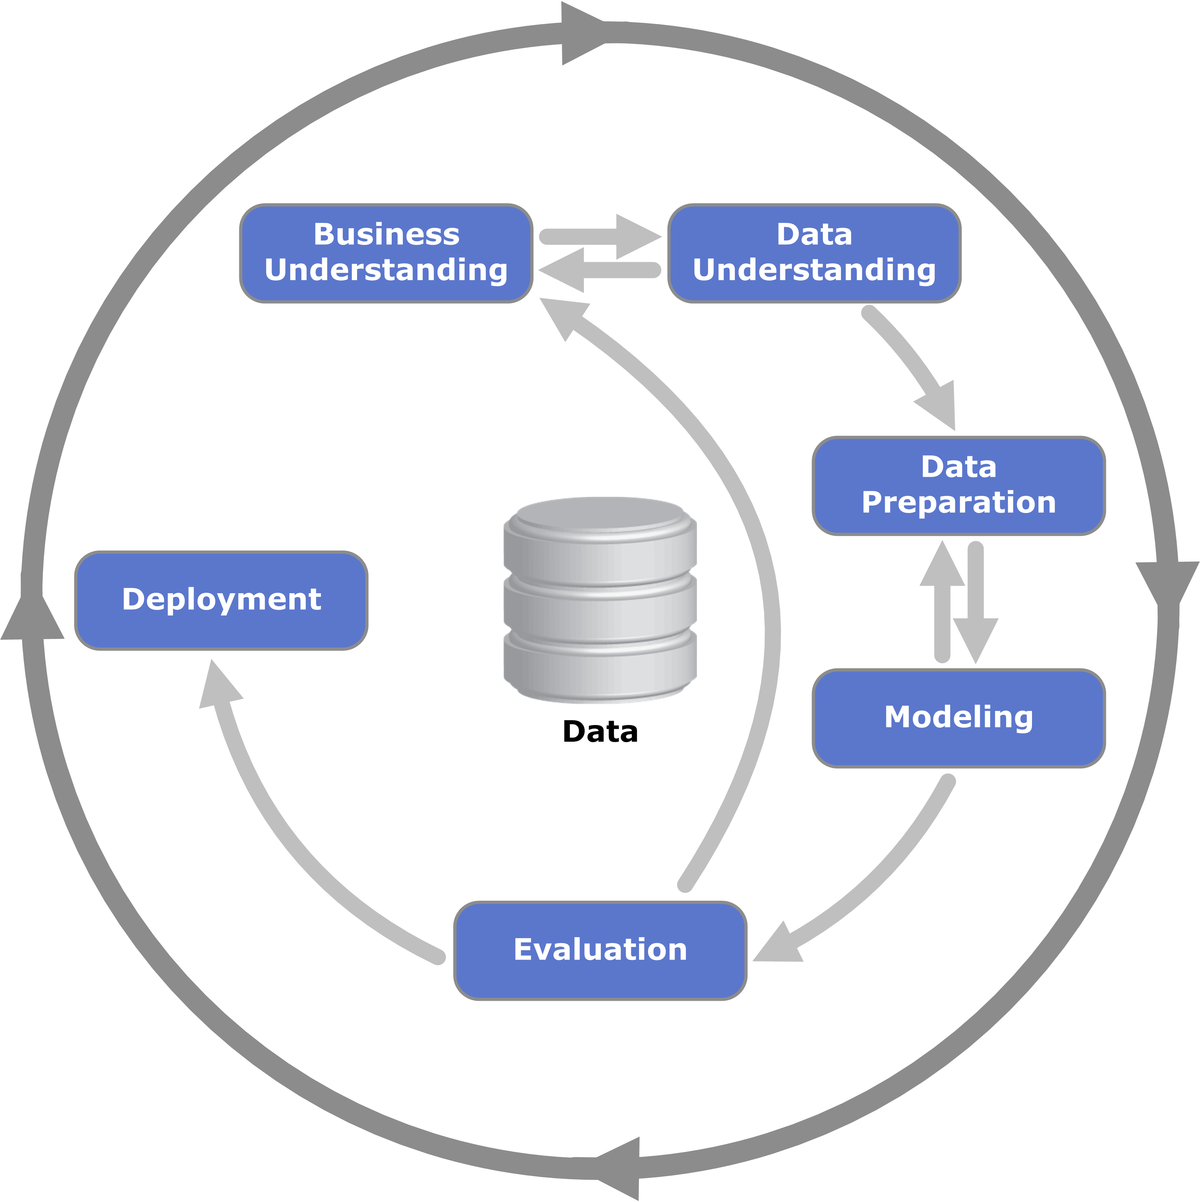
\includegraphics[width=0.35\textwidth]{crispdm.png} % Ajusta el tamaño con width o height
		\caption{Metodología CRISP-DM} % Texto del caption
		\label{fig:crispdm} % Etiqueta para referenciar la imagen
	\end{figure}
	
	
	El método CRISP-DM (Cross Industry Standard Process for Data Mining) se aplicó de la siguiente manera en el desarrollo de este proyecto de minería de textos:
	
	\subsubsection{Comprensión del Negocio}
	El objetivo principal del proyecto es analizar las opiniones y reacciones ciudadanas expresadas en redes sociales durante los debates y el día de las elecciones presidenciales de México 2024. Se busca identificar sentimientos (positivo, negativo y neutral) y temas principales asociados a los candidatos, así como las diferencias entre plataformas (YouTube y X). Este análisis permitirá comprender mejor las dinámicas sociales y la percepción pública de los candidatos.
	
	\subsubsection{Comprensión de los Datos}
	Se recopilaron dos conjuntos de datos:
	\begin{itemize}
		\item \textbf{YouTube:} Comentarios de los debates presidenciales (9,392 registros), incluyendo atributos como usuario, comentario, canal, número de "me gusta" y fecha.
		\item \textbf{X:} Publicaciones realizadas durante el día de las elecciones (2,486 registros), con atributos como usuario, hora de publicación y contenido textual.
	\end{itemize}
	Se realizó una exploración inicial para identificar datos irrelevantes, valores faltantes y posibles inconsistencias.
	
	\subsubsection{Preparación de los Datos}
	Los datos fueron limpiados eliminando duplicados, comentarios vacíos y símbolos no alfabéticos irrelevantes. Además, se realizó un proceso de tokenización, lematización y eliminación de palabras vacías (\textit{stopwords}) para estandarizar el texto. En esta etapa también se añadió una columna de sentimiento, calculada utilizando un modelo preentrenado de análisis de sentimientos.
	
	\subsubsection{Modelado}
	Para el análisis de sentimientos, se utilizó el modelo preentrenado BETO, especializado en español. Este modelo fue ajustado mediante \textit{fine-tuning} con los datos recopilados, adaptándolo al lenguaje manejado en un contexto electoral en redes sociales. 
	
	Para el modelado de tópicos, se emplearon los \textit{embeddings} generados por BETO, y se aplicó reducción de dimensionalidad mediante PCA (\textit{Principal Component Analysis}). Finalmente, se utilizó el algoritmo de agrupamiento K-means para identificar y clasificar los tópicos principales.
	
	\subsubsection{Evaluación}
	Los resultados del análisis de sentimientos se evaluaron utilizando la matriz de confusión, calculando métricas como precisión, \textit{recall} y F1-score para cada categoría de sentimiento. Para la evaluación del modelado de tópicos, se utilizó el coeficiente de silueta para medir la cohesión y separación de los clusters generados, asegurando la calidad del agrupamiento.
	
	\subsubsection{Despliegue}
	Los resultados del análisis se presentaron en forma de gráficos y visualizaciones interactivas que muestran:
	\begin{itemize}
		\item Distribución de sentimientos por candidato y plataforma.
		\item Evolución de opiniones durante el proceso electoral.
		\item Comparación entre los temas principales discutidos en YouTube y X.
	\end{itemize}
	Estas visualizaciones permiten una interpretación clara y útil para el público interesado en el análisis político y social.
	
	
	\subsection{Descripción de las Variables del Conjunto de Datos}
	
	A continuación, se presenta la descripción detallada de las variables contenidas en el conjunto de datos utilizado en este estudio. La tabla incluye numeración, nombre de la variable, significado, tipo de dato y dominio de valores.
	
	\begin{table}[h]
		\centering
		\begin{tabular}{|c|l|p{6cm}|l|p{4cm}|}
			\hline
			\textbf{Núm.} & \textbf{Variable} & \textbf{Significado} & \textbf{Tipo de Dato} & \textbf{Dominio de Valores} \\
			\hline
			1 & \texttt{num\_debate} & Número del debate presidencial en el que se realizó el comentario. & Entero & \{1, 2, 3\} \\
			\hline
			2 & \texttt{canal} & Nombre del canal de YouTube donde se transmitió el debate. & Cadena de texto & Cualquier canal reconocido (e.g., \textit{Milenio}, \textit{Nmás}). \\
			\hline
			3 & \texttt{username} & Nombre de usuario que realizó el comentario en la plataforma. & Cadena de texto & Texto alfanumérico. \\
			\hline
			4 & \texttt{fecha} & Fecha en la que se publicó el comentario. & Fecha & Formato DD/MM/AAAA. \\
			\hline
			5 & \texttt{comentario} & Contenido textual del comentario realizado por el usuario. & Cadena de texto & Cualquier texto. \\
			\hline
			6 & \texttt{num\_likes} & Número de "me gusta" que recibió el comentario. & Entero & \{0, 1, 2, \dots\} \\
			\hline
		\end{tabular}
		\caption{Descripción de las variables del conjunto de datos de comentarios en YouTube.}
		\label{tab:variables_dataset}
	\end{table}
	
	\begin{table}[h]
		\centering
		\begin{tabular}{|c|l|p{5cm}|l|p{4cm}|}
			\hline
			\textbf{Núm.} & \textbf{Variable} & \textbf{Significado} & \textbf{Tipo de Dato} & \textbf{Dominio de Valores} \\
			\hline
			1 & \texttt{User} & Nombre del usuario que publicó el tweet. & Cadena de texto & Texto alfanumérico. \\
			\hline
			2 & \texttt{arroba} & Handle del usuario precedido por ``@''. & Cadena de texto & Texto alfanumérico (e.g., \texttt{@usuario}). \\
			\hline
			3 & \texttt{hora\_publicación} & Hora en la que se publicó el tweet. & Hora & Formato HH:MM (24 horas). \\
			\hline
			4 & \texttt{publicación} & Contenido textual del tweet. & Cadena de texto & Texto libre (e.g., comentarios, reacciones). \\
			\hline
		\end{tabular}
		\caption{Descripción de las variables del conjunto de datos de X.}
		\label{tab:variables_dataset_X}
	\end{table}
	
	
	
	\subsection{Tareas de Minería de Datos}
	
	Para realizar el análisis de los comentarios recopilados en redes sociales durante los debates y el día de la elección presidencial, se utilizarán los siguientes algoritmos y técnicas:
	
	\subsubsection{Análisis del tipo de sentimiento}
	
	El análisis de sentimientos tiene como objetivo clasificar los comentarios en categorías como positivo, negativo y neutral. Para esta tarea se empleará el siguiente enfoque:
	
	\begin{itemize}
		\item \textbf{BETO con Fine-Tuning}: Este modelo preentrenado en español será ajustado mediante \textit{fine-tuning} para capturar patrones textuales específicos del contexto electoral. Este enfoque permite clasificaciones más precisas al considerar dependencias contextuales entre las palabras, adaptándolo al lenguaje y las emociones presentes en las redes sociales.
	\end{itemize}
	
	
	
	\subsubsection{Análisis de Tópicos}
	
	El análisis de tópicos busca identificar los temas predominantes en los comentarios. Para esta tarea, se implementará una combinación de representaciones de palabras, reducción de dimensionalidad y agrupamiento:
	
	\begin{itemize}
		\item \textbf{Embeddings de Palabras}: Se utilizarán los embeddings de BETO para generar representaciones vectoriales densas de las palabras, capturando relaciones semánticas y contextuales en el corpus de texto.
		\item \textbf{Reducción de Dimensionalidad con PCA}: Antes de aplicar el agrupamiento, se utilizará el análisis de componentes principales (PCA, por sus siglas en inglés) para reducir la dimensionalidad de los embeddings generados, conservando las características más relevantes y mejorando la eficiencia del algoritmo.
		\item \textbf{K-means}: Sobre los embeddings reducidos, se aplicará el algoritmo de agrupamiento K-means para identificar grupos de comentarios relacionados con tópicos similares.
	\end{itemize}
	
	Esta combinación permitirá descubrir los temas más relevantes dentro de los comentarios analizados, proporcionando una visión más clara de las discusiones predominantes en las plataformas sociales.
	
	\subsection{Modelo del Framework de Desarrollo}
	
	\begin{figure}[h!] % 'h!' posiciona la imagen cerca del texto relacionado
		\centering
		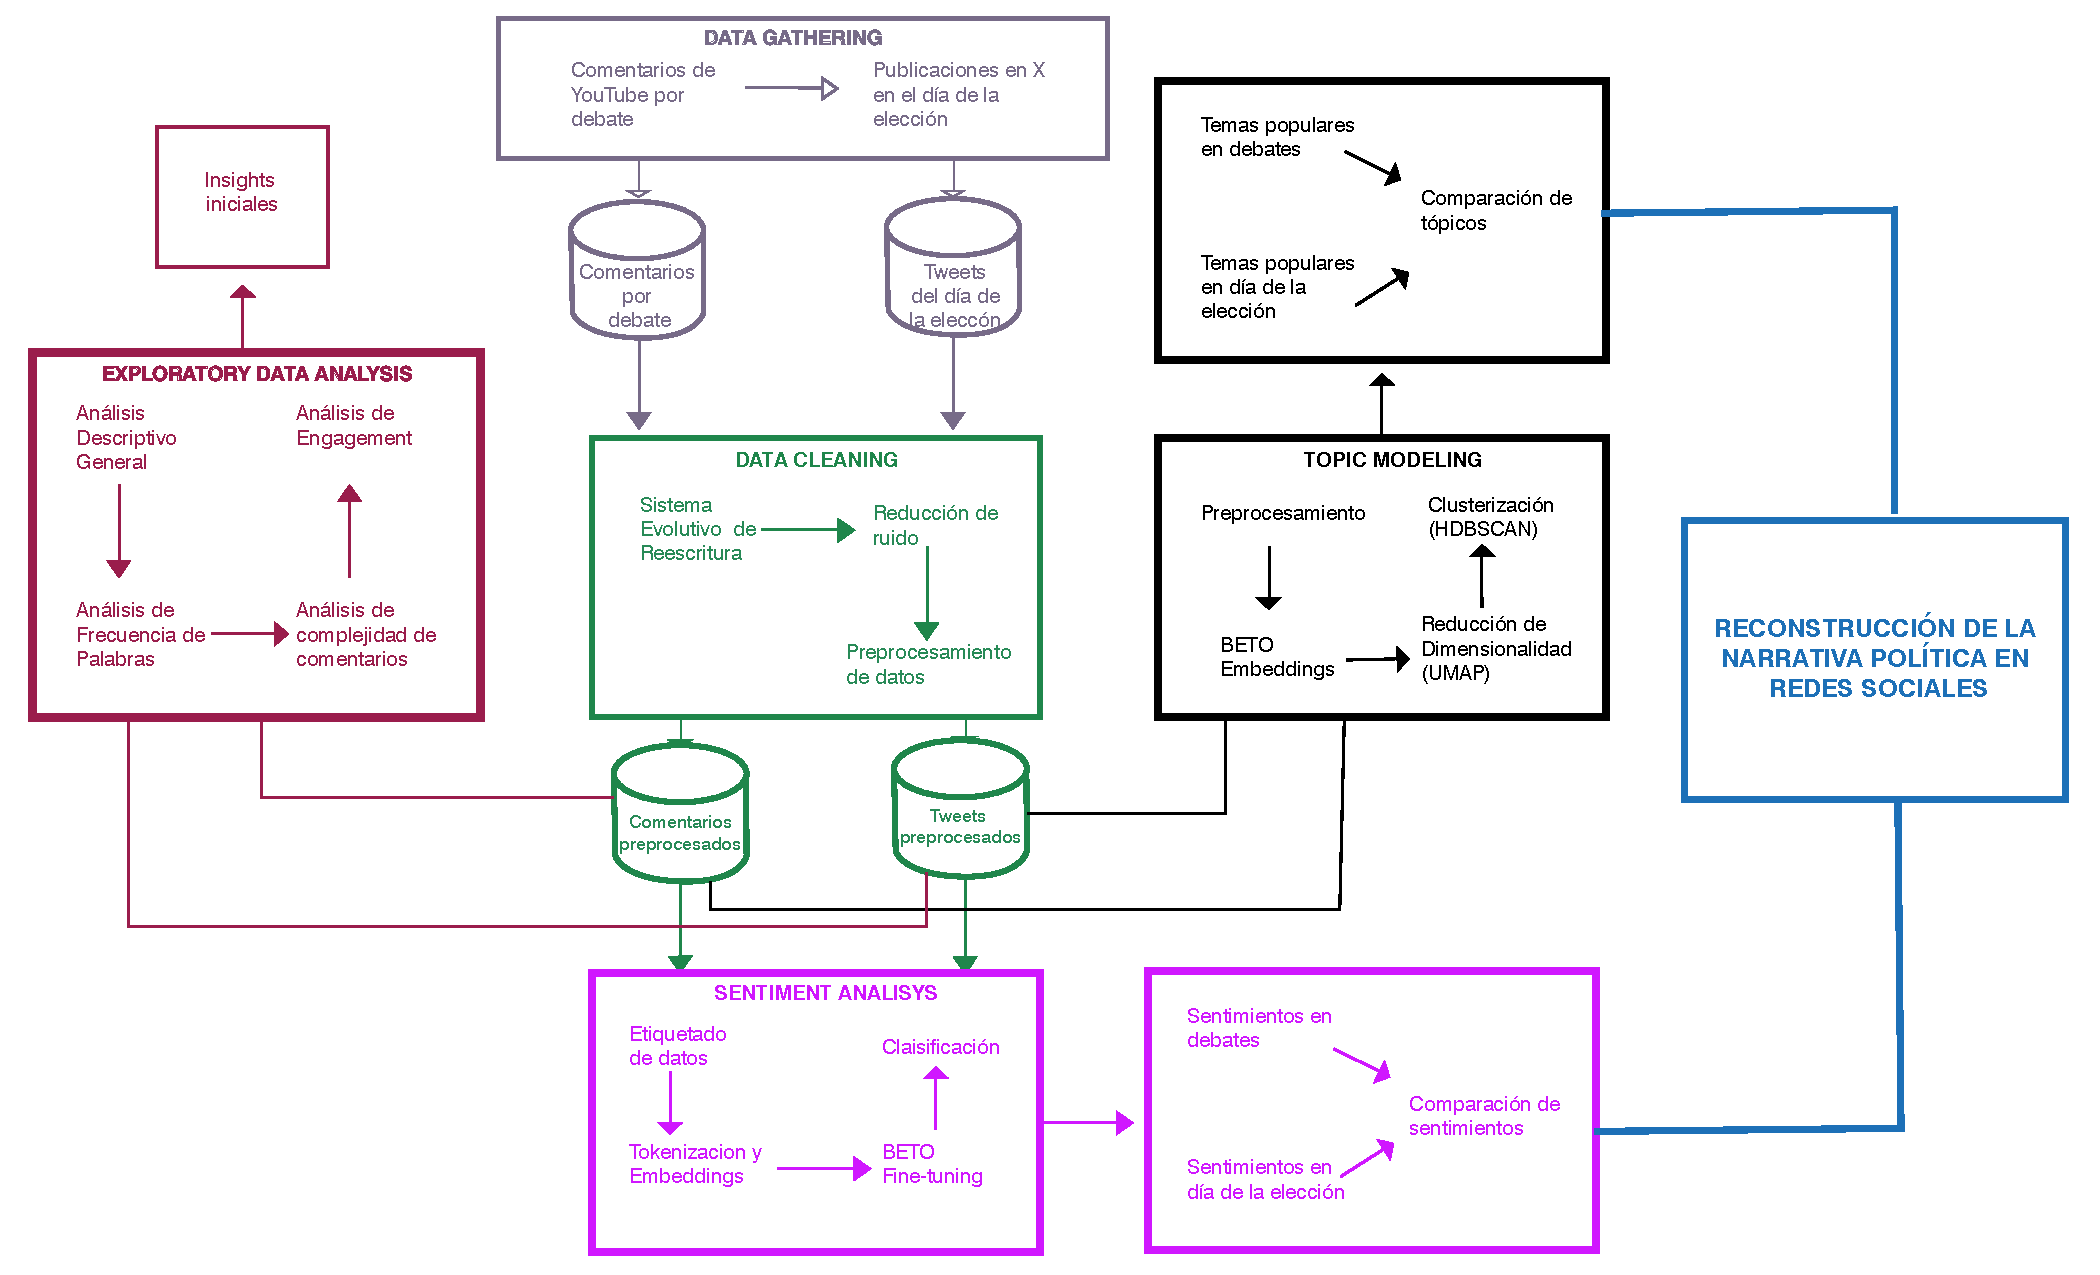
\includegraphics[width=0.8\textwidth]{diagrama.pdf} % Ajusta el tamaño con width o height
		\caption{Framework de Deasarrollo} % Texto del caption
		\label{fig:framework} % Etiqueta para referenciar la imagen
	\end{figure}
	
	
	\section{Resultados}
	
	En esta sección se presentará una descripción de los resultados obtenidos en cada una de las etapas descritas en el diagrama del proceso de análisis. De esta manera, se mostrara cómo cada etapa contribuye a generar \textit{insights} sobre las opiniones y temas predominantes expresados durante los debates presidenciales y el día de la elección en las plataformas de redes sociales analizadas.
	
	\subsection{Limpieza de Datos}
	
	Uno de los principales retos al trabajar con datos textuales provenientes de redes sociales es la calidad inconsistente del contenido. En este proyecto, se identificaron varios problemas específicos que complican el análisis automatizado:
	
	\begin{itemize}
		\item \textbf{Mala escritura y faltas de ortografía:} Los comentarios y publicaciones contienen errores ortográficos frecuentes, como palabras mal escritas, omisión de acentos y uso incorrecto de mayúsculas o minúsculas. Estos errores dificultan la tokenización y lematización, al aumentar la variabilidad de las palabras.
		
		\item \textbf{Jerga mexicana y expresiones coloquiales:} Muchos usuarios emplean mexicanismos y modismos propios del contexto cultural, como “chido”, “gacho” o “fifí”. Estas expresiones no están presentes en la mayoría de los diccionarios estándar, lo que limita el desempeño de los modelos preentrenados en el análisis semántico.
		
		\item \textbf{Uso de groserías y lenguaje ofensivo:} Palabras altisonantes como “pendejo” o “culero” son comunes en las discusiones políticas en redes sociales. Estas palabras no solo tienen connotaciones emocionales fuertes, sino que también presentan múltiples variantes (e.g., \textit{pendejo}, \textit{culero}), lo que incrementa la complejidad del análisis de sentimientos.
		
		\item \textbf{Abreviaturas y términos políticos:} Los usuarios utilizan abreviaturas y siglas para referirse a candidatos o partidos, como “AMLO”, “4T” o “PRIAN”. Además, emplean términos únicos del discurso político en México, como “chairos” y “fifís”, que requieren interpretación contextual para su correcta clasificación.
		
	\end{itemize}
	
	Estos problemas no solo dificultan el procesamiento y análisis de los textos, sino que también pueden introducir sesgos en los resultados al interpretar palabras con múltiples variantes o significados según el contexto.
	
	Para abordar estos desafíos, se implementó un \textit{sistema evolutivo de reescritura} \parencite{galindo1991sistemas}, diseñado para realizar una limpieza parcial y estandarización de los textos. 
	
	\subsubsection{Sistema Evolutivo de Reescritura}
	
	Este sistema incluye las siguientes funciones:
	\begin{itemize}
		\item Corrección automática de errores ortográficos y adición de acentos en palabras comunes.
		\item Reducción de variantes de mexicanismos y groserías a una forma estándar.
		\item Reescritura de abreviaturas y siglas, asociándolas con su significado completo en el contexto electoral.
		\item Sustitución de términos coloquiales y ofensivos por equivalentes neutros o su forma semánticamente más representativa.
	\end{itemize}
	
	Los sistemas evolutivos de reescritura se basan en la aplicación iterativa de reglas de transformación de datos para resolver problemas representados como cadenas de caracteres o bits. Un sistema de este tipo se estructura típicamente de la siguiente manera:
	
	\begin{itemize}
		\item Un conjunto de elementos de entrada (\textit{A}).
		\item Un conjunto de elementos de salida (\textit{B}).
		\item Un conjunto de reglas de reescritura (\textit{R}), definidas como $X \rightarrow Y$, donde $X \in A^*$ y $Y \in B^*$. Esto significa que $X$ puede reescribirse como $Y$.
	\end{itemize}
	
	Cada regla de reescritura especifica cómo transformar un patrón de entrada en un patrón de salida, lo que permite representar una gran variedad de problemas. Estos sistemas son evolutivos porque permiten que las reglas se actualicen dinámicamente durante el funcionamiento del sistema. Si se encuentra un caso nuevo que no está cubierto por las reglas existentes, el sistema puede solicitar información al usuario o a un experto para generar una nueva regla que se almacena automáticamente \parencite{galindo1991sistemas}.
	
	\textbf{Funcionamiento básico}:
	\begin{enumerate}
		\item El sistema compara la entrada con las reglas almacenadas.
		\item Si encuentra una coincidencia, aplica la transformación especificada en la regla.
		\item Si no encuentra una coincidencia, solicita una nueva regla, que luego se añade al sistema.
		\item Este proceso permite que el sistema \textit{aprenda} y mejore con el tiempo, adaptándose a nuevos escenarios y ampliando su base de conocimiento.
	\end{enumerate}
	
	
	Como primer paso para implementar el sistema evolutivo de reescritura, construimos una bolsa inicial de 136 palabras que incluyen términos coloquiales, términos de política mexicana, groserías y abreviaturas comunes en redes sociales. Este conjunto se elaboró a partir de una revisión exhaustiva de los comentarios y publicaciones del conjunto de datos. Algunos ejemplos de palabras incluidas son:
	
	\begin{table}[H]
		\centering
		\resizebox{\textwidth}{!}{%
			\begin{tabular}{|l|c|c|l|l|}
				\hline
				\textbf{Palabra} & \textbf{Nivel de Intensidad} & \textbf{Sentimiento Asociado} & \textbf{Categoría} & \textbf{Comentarios} \\ \hline
				chairo & 3 & negativo & insulto & término despectivo contra votantes de izquierda \\ \hline
				fifi & 3 & negativo & insulto & término usado contra votantes de derecha \\ \hline
				asqueroso & 4 & negativo & adjetivo & término coloquial usado para describir desagrado \\ \hline
				mamón & 3 & negativo & insulto & usado para descalificar \\ \hline
			\end{tabular}%
		}
		\caption{Ejemplo de palabras incluidas en la bolsa inicial.}
		\label{tab:bolsa_palabras}
	\end{table}
	
	
	El propósito de esta bolsa de palabras es servir como base para el sistema evolutivo de reescritura. Este sistema aplica las siguientes acciones sobre los textos:
	\begin{itemize}
		\item \textbf{Estandarización:} Palabras con múltiples variantes (e.g., "fifi", "fifí") se reducen a una forma única para minimizar ruido semántico.
		\item \textbf{Limpieza:} Groserías, abreviaturas y errores ortográficos son corregidos, con el fin de mejorar la legibilidad y procesabilidad del texto.
	\end{itemize}
	
	Al utilizar esta bolsa de palabras como referencia inicial, el sistema evolutivo de reescritura es capaz de minimizar el ruido en los textos procesados. Esto facilita que el modelo de lenguaje interprete y analice los datos de manera más efectiva, reduciendo la ambigüedad y los sesgos que pueden surgir debido al uso de jerga o expresiones coloquiales.
	
	El sistema evolutivo no solo se limita a esta bolsa inicial; a través de su diseño, puede adaptarse dinámicamente, incorporando nuevas palabras y reglas según se identifiquen durante el análisis. De esta manera, se garantiza que el texto procesado sea progresivamente más limpio y útil para las etapas posteriores de minería de textos y modelado \parencite{galindo1991sistemas}.
	
	\begin{figure}[h!] % 'h!' posiciona la imagen cerca del texto relacionado
		\centering
		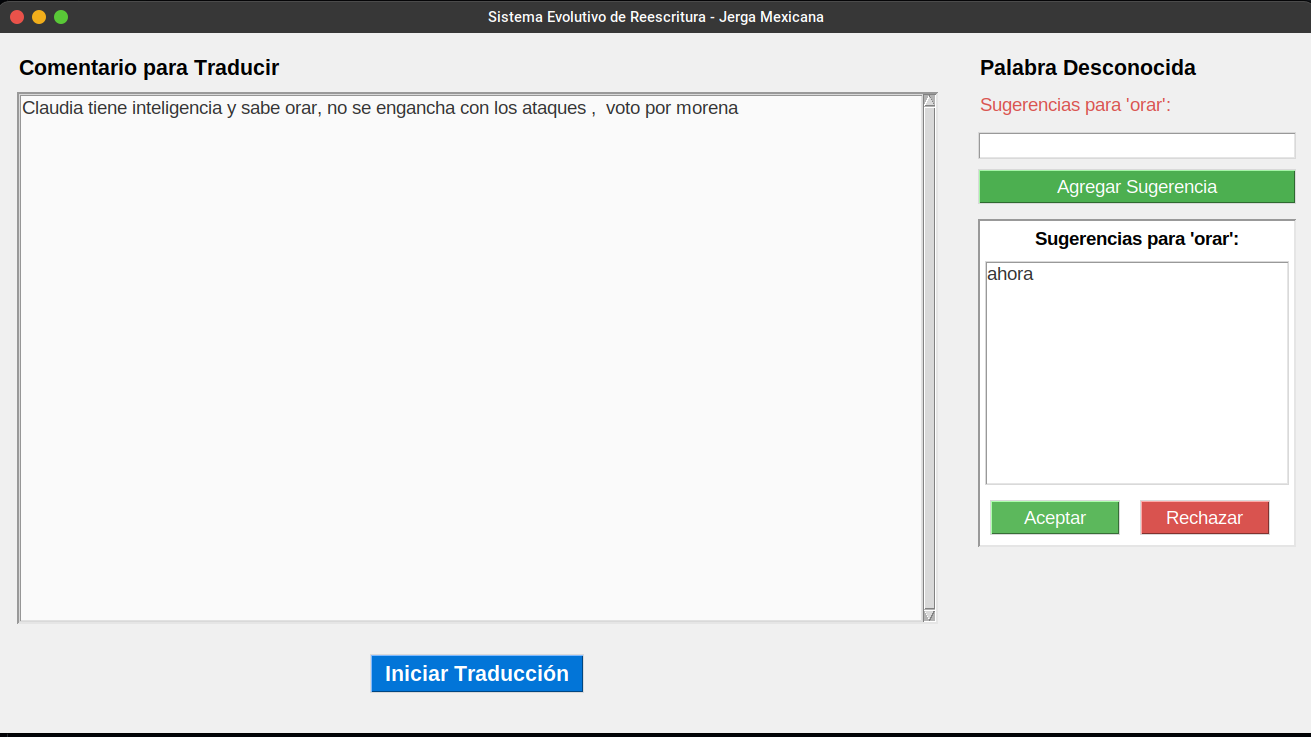
\includegraphics[width=0.7\textwidth]{evolutivo.png} % Ajusta el tamaño con width o height
		\caption{Sistema Evolutivo de Reescritura} % Texto del caption
		\label{fig:evolutivo} % Etiqueta para referenciar la imagen
	\end{figure}
	
	Como resultado de la implementación del sistema evolutivo de reescritura, se logró una reducción del ruido en los textos procesados. Este sistema permitió estandarizar palabras con múltiples variantes, corregir errores ortográficos, reemplazar términos coloquiales, y normalizar abreviaturas utilizadas en el contexto político y social. Tras aplicar este proceso, se generaron versiones actualizadas de los dos conjuntos de datos originales, incorporando una nueva columna denominada \textbf{comentario\_editado}. Esta columna contiene los textos procesados y limpios, listos para ser utilizados en las siguientes etapas de análisis.
	
	\subsubsection{Preprocesamiento de Datos}
	
	Ahora, para continuar con el proceso de minería de textos se aplicó la metodología de preprocesamiento de datos descrita por Gelbukh \parencite{gelbukh2003procesamiento}, que incluye las siguientes etapas fundamentales:
	
	\begin{itemize}
		\item \textbf{Conversión a minúsculas:} Todos los textos fueron convertidos a letras minúsculas para evitar que diferencias de mayúsculas y minúsculas afecten la agrupación de palabras similares.
		
		\item \textbf{Eliminación de emojis y caracteres no textuales:} Se eliminaron los emojis, caracteres especiales y elementos visuales, ya que no aportan información significativa al análisis lingüístico.
		
		\item \textbf{Eliminación de URLs:} Las direcciones web fueron removidas, dado que no representan contenido relevante para el análisis semántico.
		
		\item \textbf{Eliminación de signos de puntuación:} Se eliminaron los signos de puntuación para simplificar la tokenización y garantizar que las palabras sean procesadas sin interferencias.
		
		\item \textbf{Tokenización:} Este proceso consiste en dividir el texto en sus componentes básicos, llamados tokens, que usualmente corresponden a palabras individuales.
		
		\item \textbf{Eliminación de stopwords:} Las palabras vacías, como artículos, preposiciones y conjunciones (por ejemplo, \textit{y}, \textit{de}, \textit{el}), que no aportan significado semántico, fueron eliminadas.
		
		\item \textbf{Lematización:} Cada palabra se redujo a su forma base o lema, eliminando variaciones morfológicas. Por ejemplo, palabras como \textit{comiendo} y \textit{comerán} fueron convertidas a su forma base \textit{comer}.
	\end{itemize}
	
	\subsection{Análisis Exploratorio de Datos}
	
	\subsubsection{Análisis Descriptivo General}
	En esta sección, se presentan las características generales de los datos recopilados, proporcionando una visión inicial de las interacciones en redes sociales relacionadas con los debates presidenciales y el día de la elección en México 2024. Se analizan las distribuciones de comentarios y publicaciones por fecha y hora, así como la frecuencia de menciones a los principales candidatos en las plataformas de YouTube y X.
	
	El análisis exploratorio incluye un conteo de las menciones explícitas a los candidatos Claudia Sheinbaum, Xóchitl Gálvez y Jorge Álvarez Maynez en los comentarios y publicaciones recopilados. Este análisis permite identificar la relevancia de cada candidato en las discusiones y ofrece una perspectiva preliminar sobre las tendencias y temas predominantes en las conversaciones sociales.
		
	\begin{figure}[h!]
		\centering
		\begin{minipage}{0.49\textwidth} % Mitad del ancho de la página
			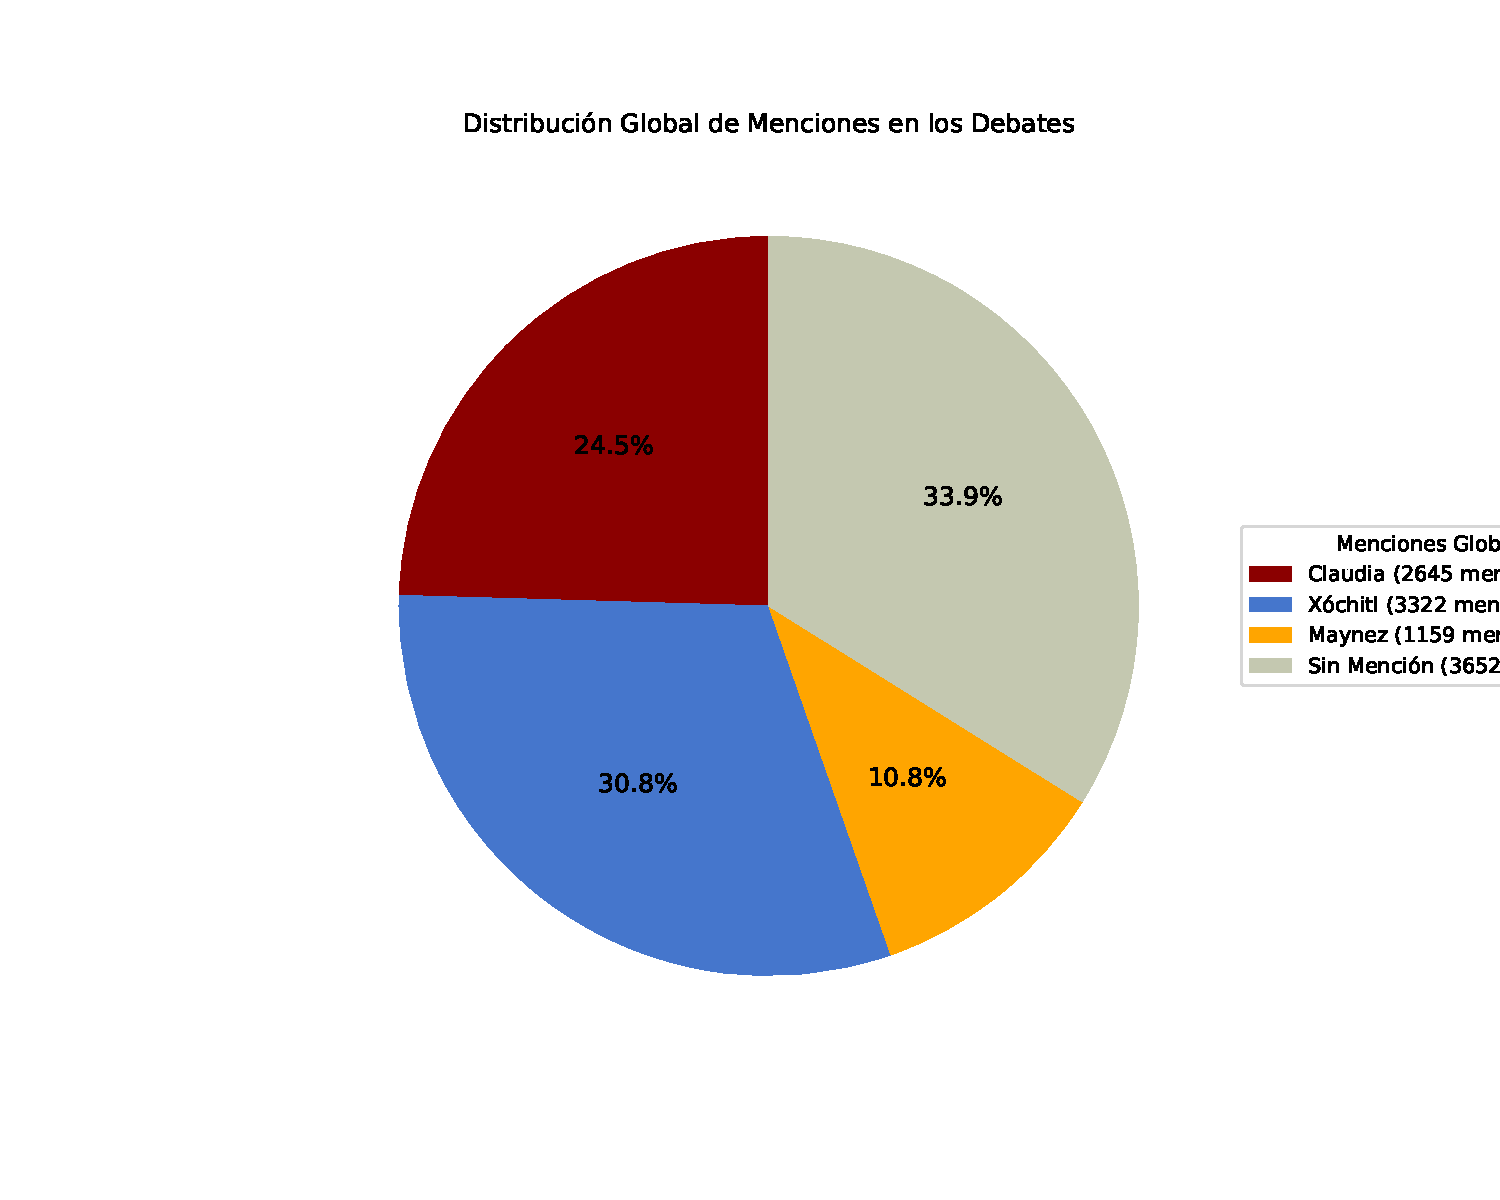
\includegraphics[width=\linewidth]{grafica_global_debates.pdf} 
			\caption{Distribución Global de Menciones en Debates}
			\label{fig:globalDebates}
		\end{minipage}
		\hfill % Espacio flexible entre las dos imágenes
		\begin{minipage}{0.49\textwidth}
			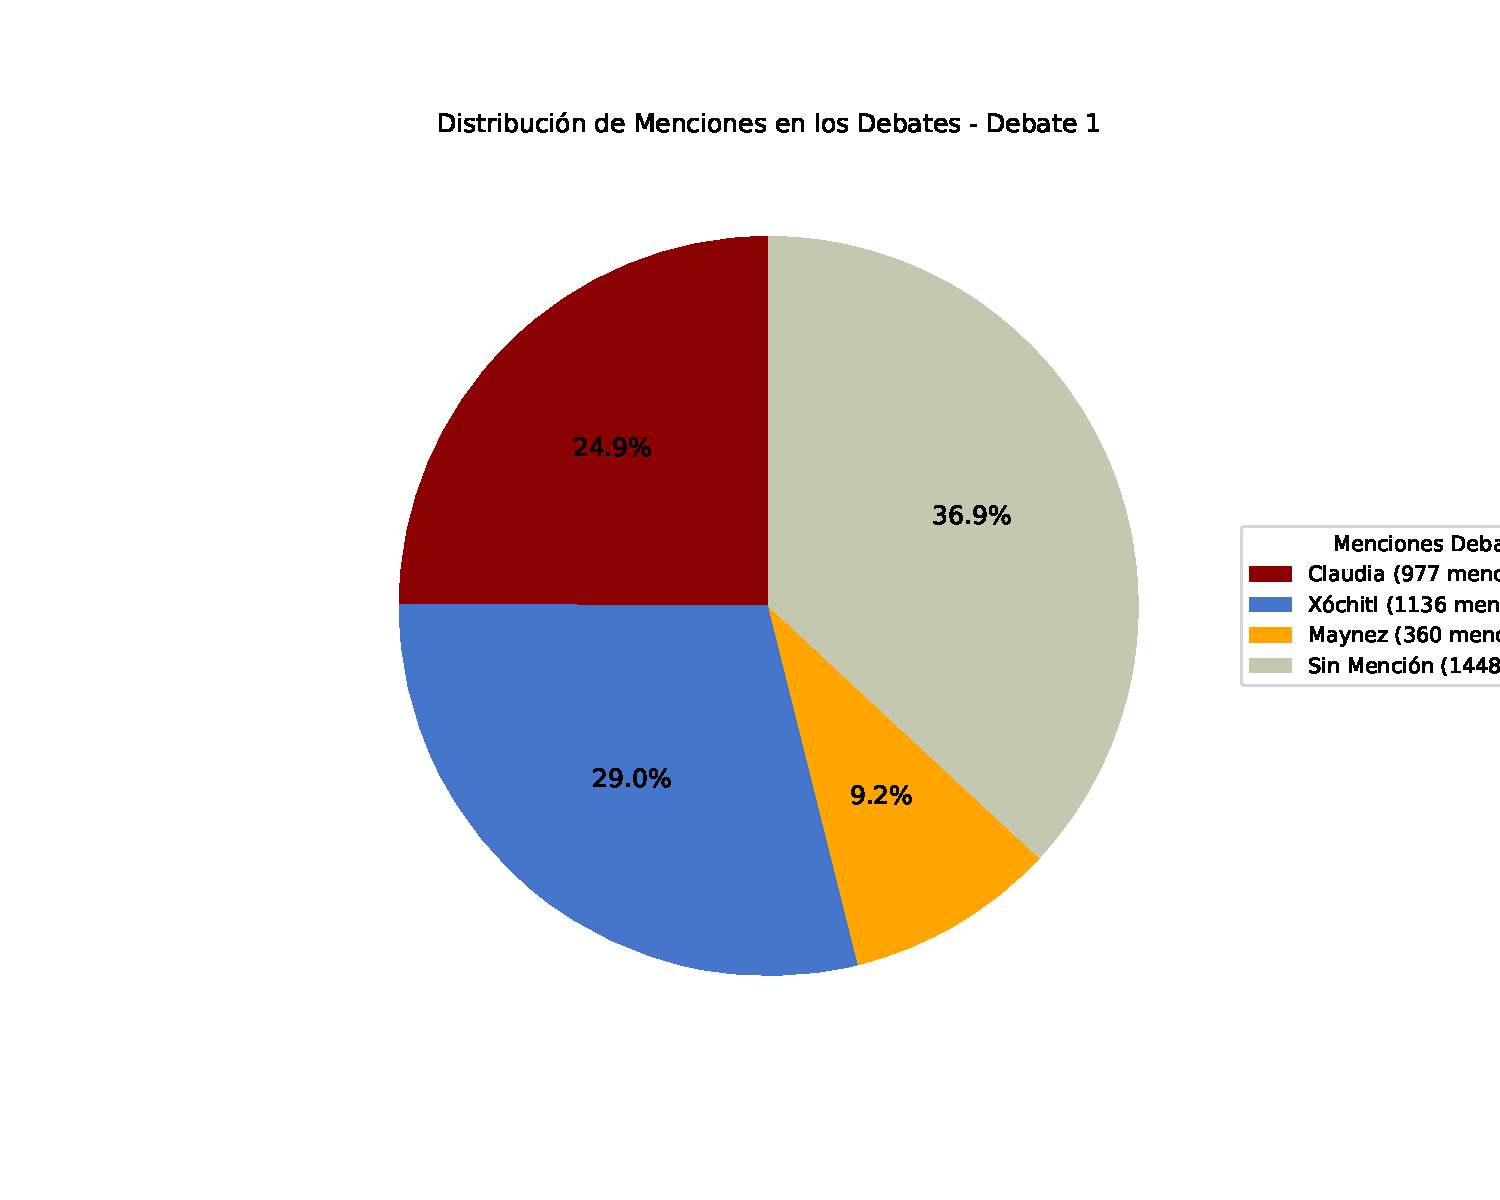
\includegraphics[width=\linewidth]{grafica_debate1.pdf}
			\caption{Distribución en el primer debate}
			\label{fig:distrDebate1}
		\end{minipage}
	\end{figure}
	
	\begin{figure}[h!]
		\centering
		\begin{minipage}{0.49\textwidth} % Mitad del ancho de la página
			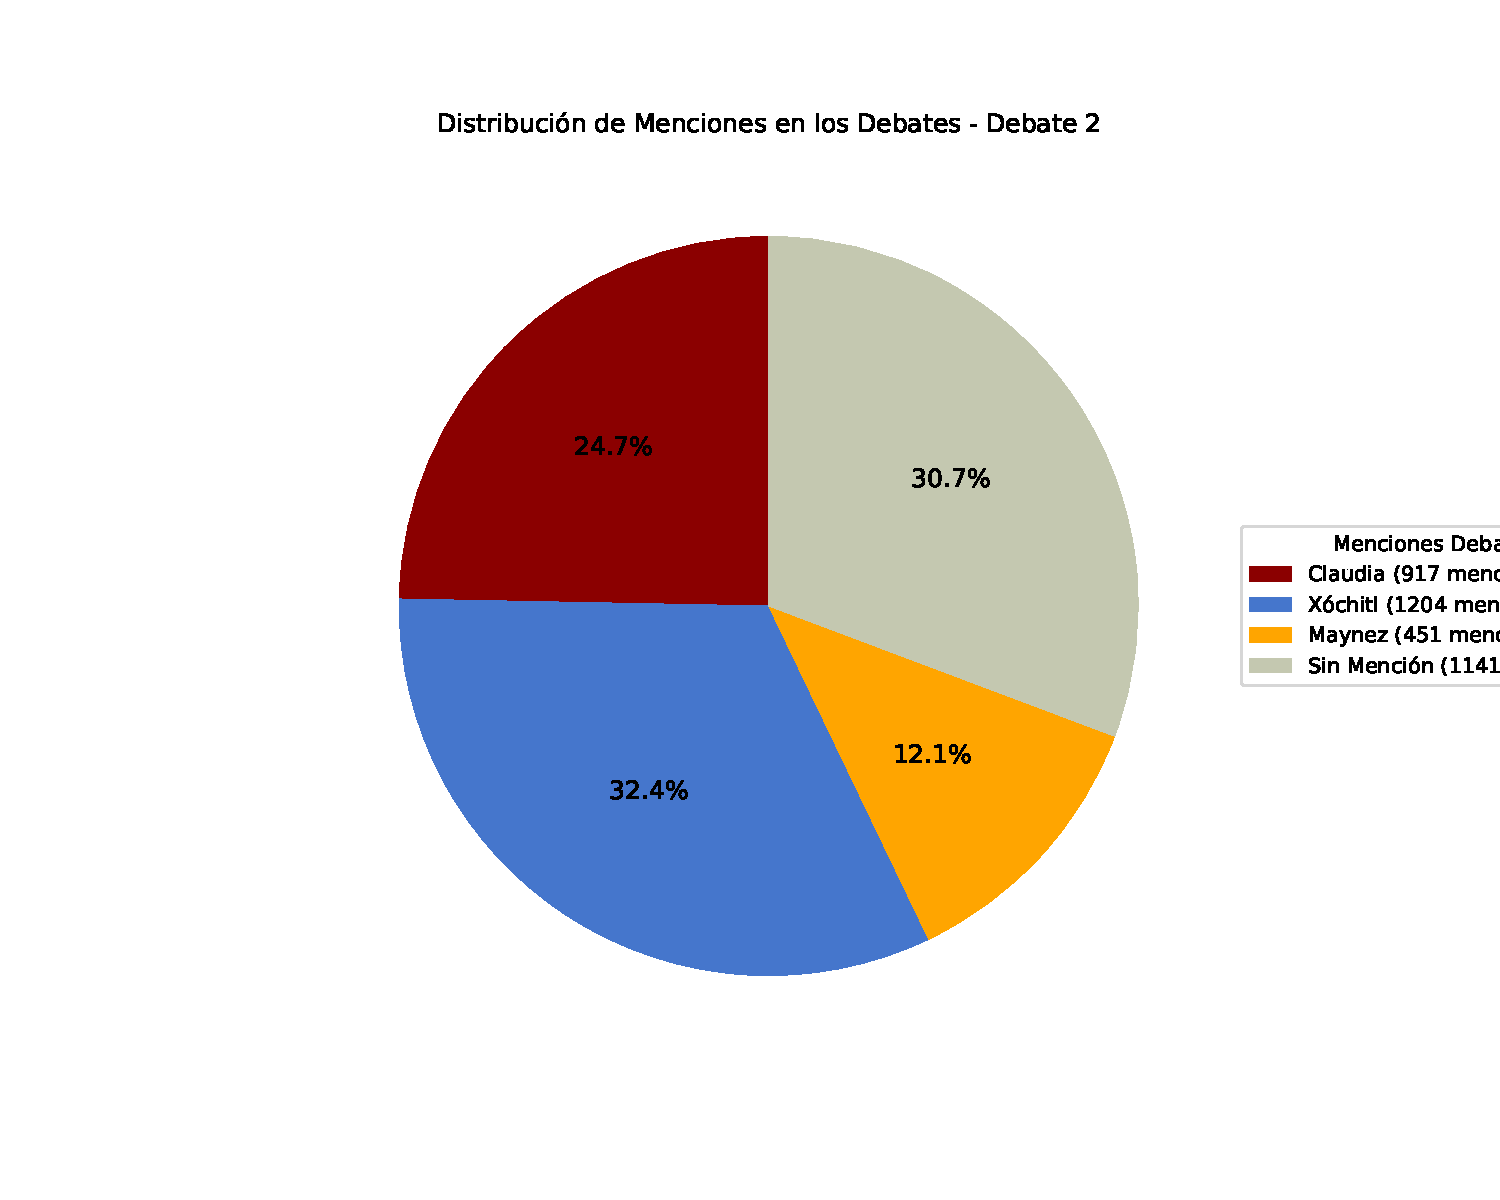
\includegraphics[width=\linewidth]{grafica_debate2.pdf} 
			\caption{Distribución en el segundo debate}
			\label{fig:distrDebate2}
		\end{minipage}
		\hfill % Espacio flexible entre las dos imágenes
		\begin{minipage}{0.49\textwidth}
			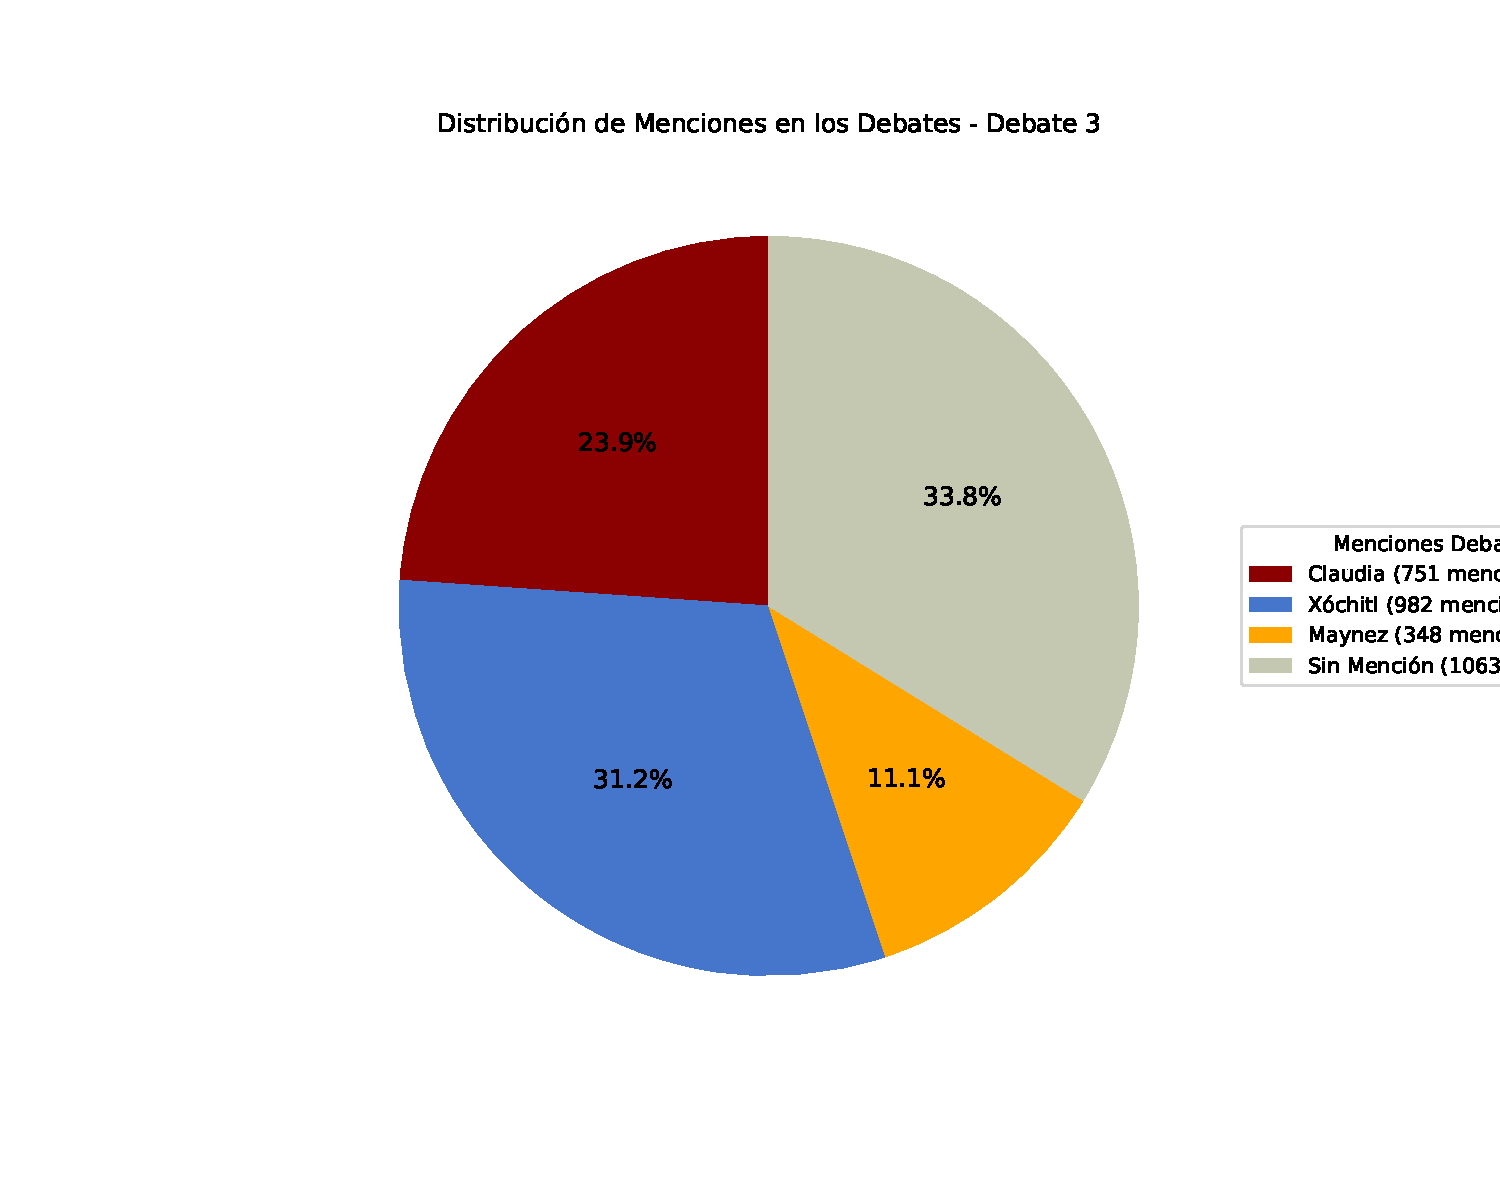
\includegraphics[width=\linewidth]{grafica_debate3.pdf}
			\caption{Distribución en el tercer debate}
			\label{fig:distrDebate3}
		\end{minipage}
	\end{figure}

	
	En el análisis global y por cada debate, se observa una tendencia constante en la distribución de menciones hacia los candidatos:
	
	\begin{itemize}
		\item \textbf{Menciones Generales:} Una proporción considerable de los comentarios no menciona a ningún candidato específico (entre 30\% y 36\% en todas las gráficas). Esto sugiere que una gran parte de las interacciones en los debates se centra en aspectos generales del evento, como la dinámica, los moderadores o los temas tratados, en lugar de los candidatos individuales.
		
		\item \textbf{Competencia entre Claudia y Xóchitl:} Claudia Sheinbaum y Xóchitl Gálvez mantienen una distribución de menciones muy equilibrada en todos los debates, con porcentajes alrededor del 24\% al 32\%. Esto refleja que ambas candidatas generaron un nivel similar de interés y discusión en las redes sociales, consolidándose como las figuras más relevantes del proceso.
		
		\item \textbf{Menor Presencia de Maynez:} Jorge Álvarez Maynez tiene una proporción significativamente menor de menciones, oscilando entre el 9\% y 12\%. Esto sugiere que su participación generó menos resonancia o interés en comparación con las otras dos candidatas.
		
		\item \textbf{Constancia entre los Debates:} Las gráficas muestran una distribución bastante estable a lo largo de los debates, lo que indica que no hubo cambios drásticos en la atención que los usuarios prestaron a cada candidato entre uno y otro evento.
	\end{itemize}

	Para realizar el análisis del día de la elección, se decidió dividir la jornada en intervalos horarios. Este enfoque permitió identificar qué candidato tuvo mayor presencia en las publicaciones realizadas por los usuarios que seguían el desarrollo de la jornada electoral. Tras el procesamiento de los datos, se obtuvieron los siguientes resultados de interacción a lo largo del día.
	
	\begin{figure}[h!]
		\centering
		\begin{minipage}{0.49\textwidth} % Mitad del ancho de la página
			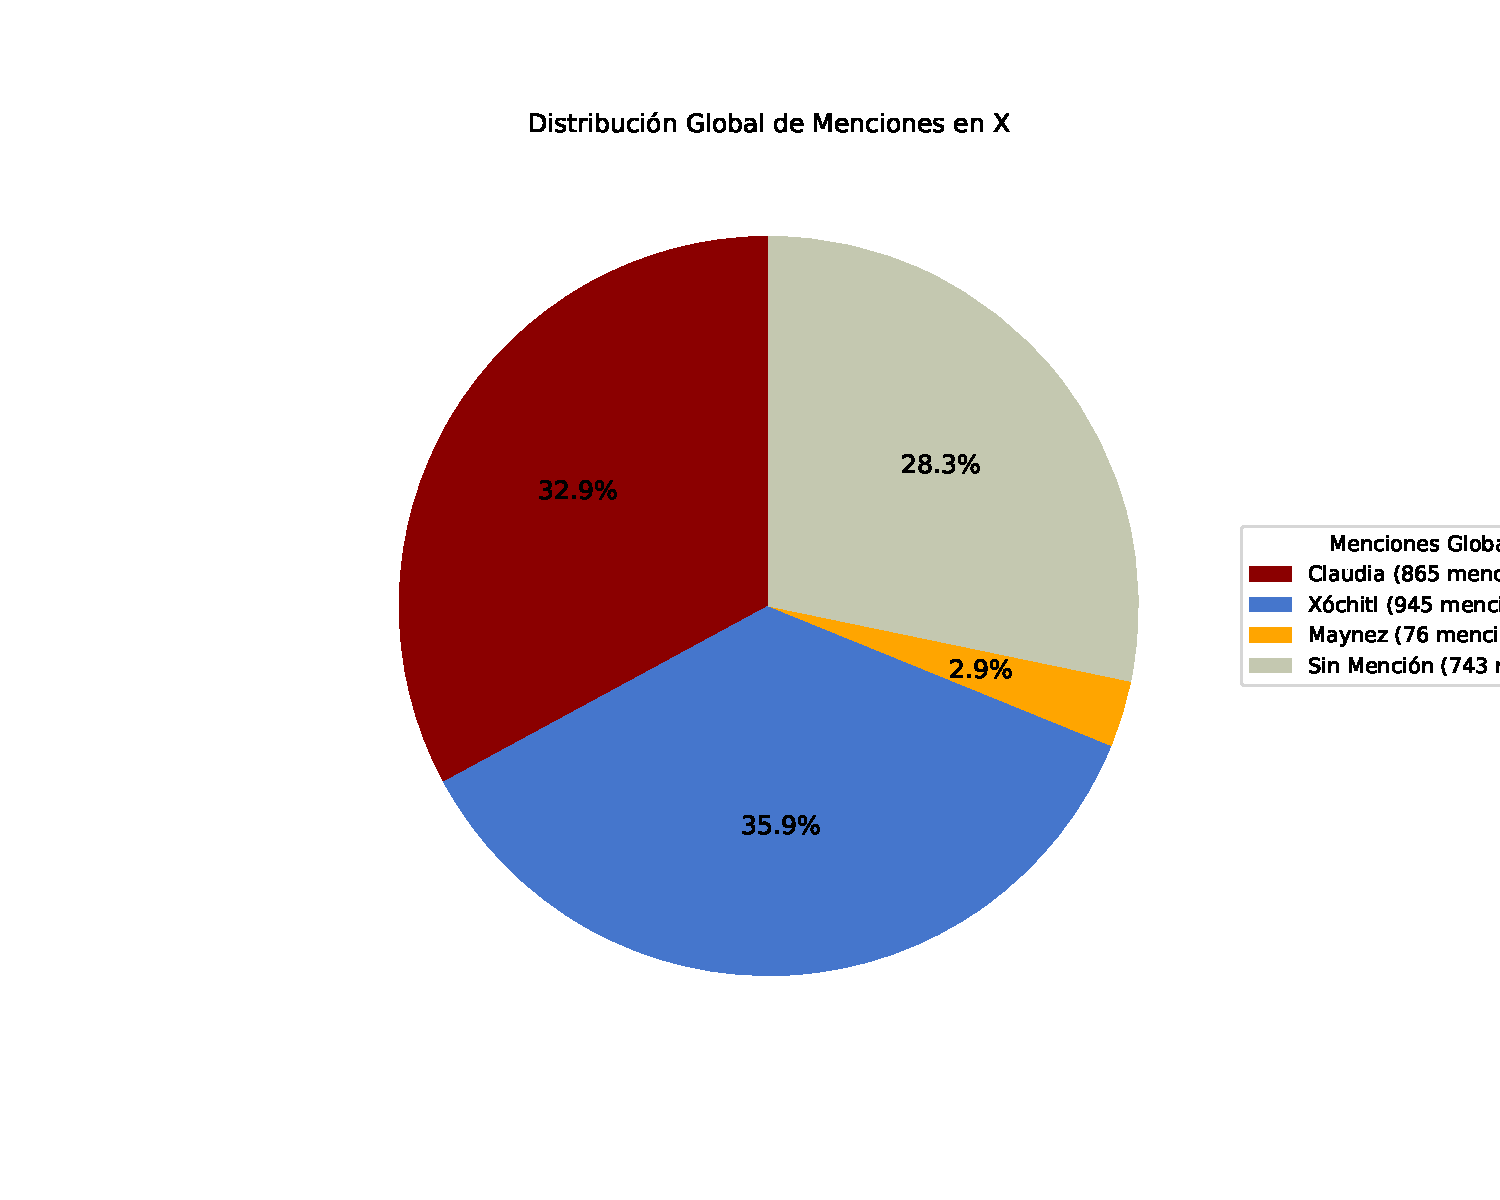
\includegraphics[width=\linewidth]{grafica_global_x.pdf} 
			\vspace{-15mm}
			\caption{Distribución Global de Menciones en el Día de la Elección}
			\label{fig:globalDiaEleccion}
		\end{minipage}
		\hfill % Espacio flexible entre las dos imágenes
		\begin{minipage}{0.49\textwidth}
			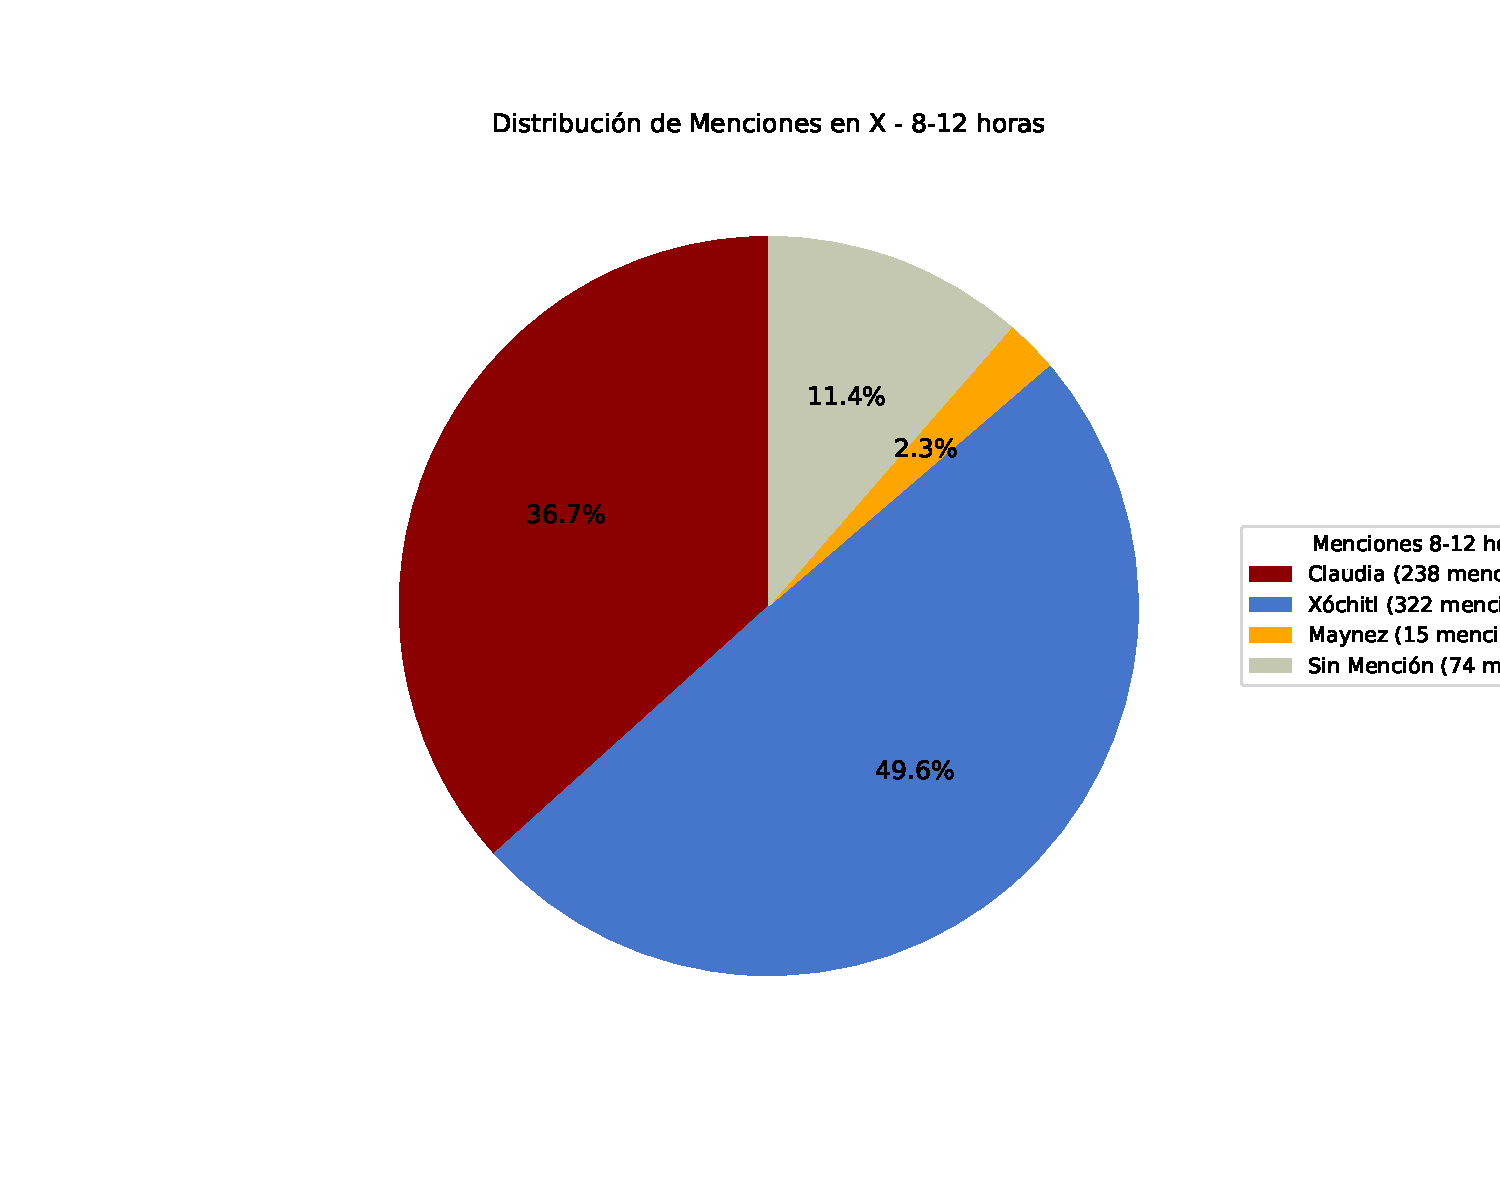
\includegraphics[width=\linewidth]{grafica_intervalo_8-12.pdf}
			\vspace{-15mm}
			\caption{Distribución de Menciones de 08:00 a 12:00}
			\label{fig:xIntervalo812}
		\end{minipage}
	\end{figure}
	
	\begin{figure}[h!]
		\centering
		\begin{minipage}{0.49\textwidth} % Mitad del ancho de la página
			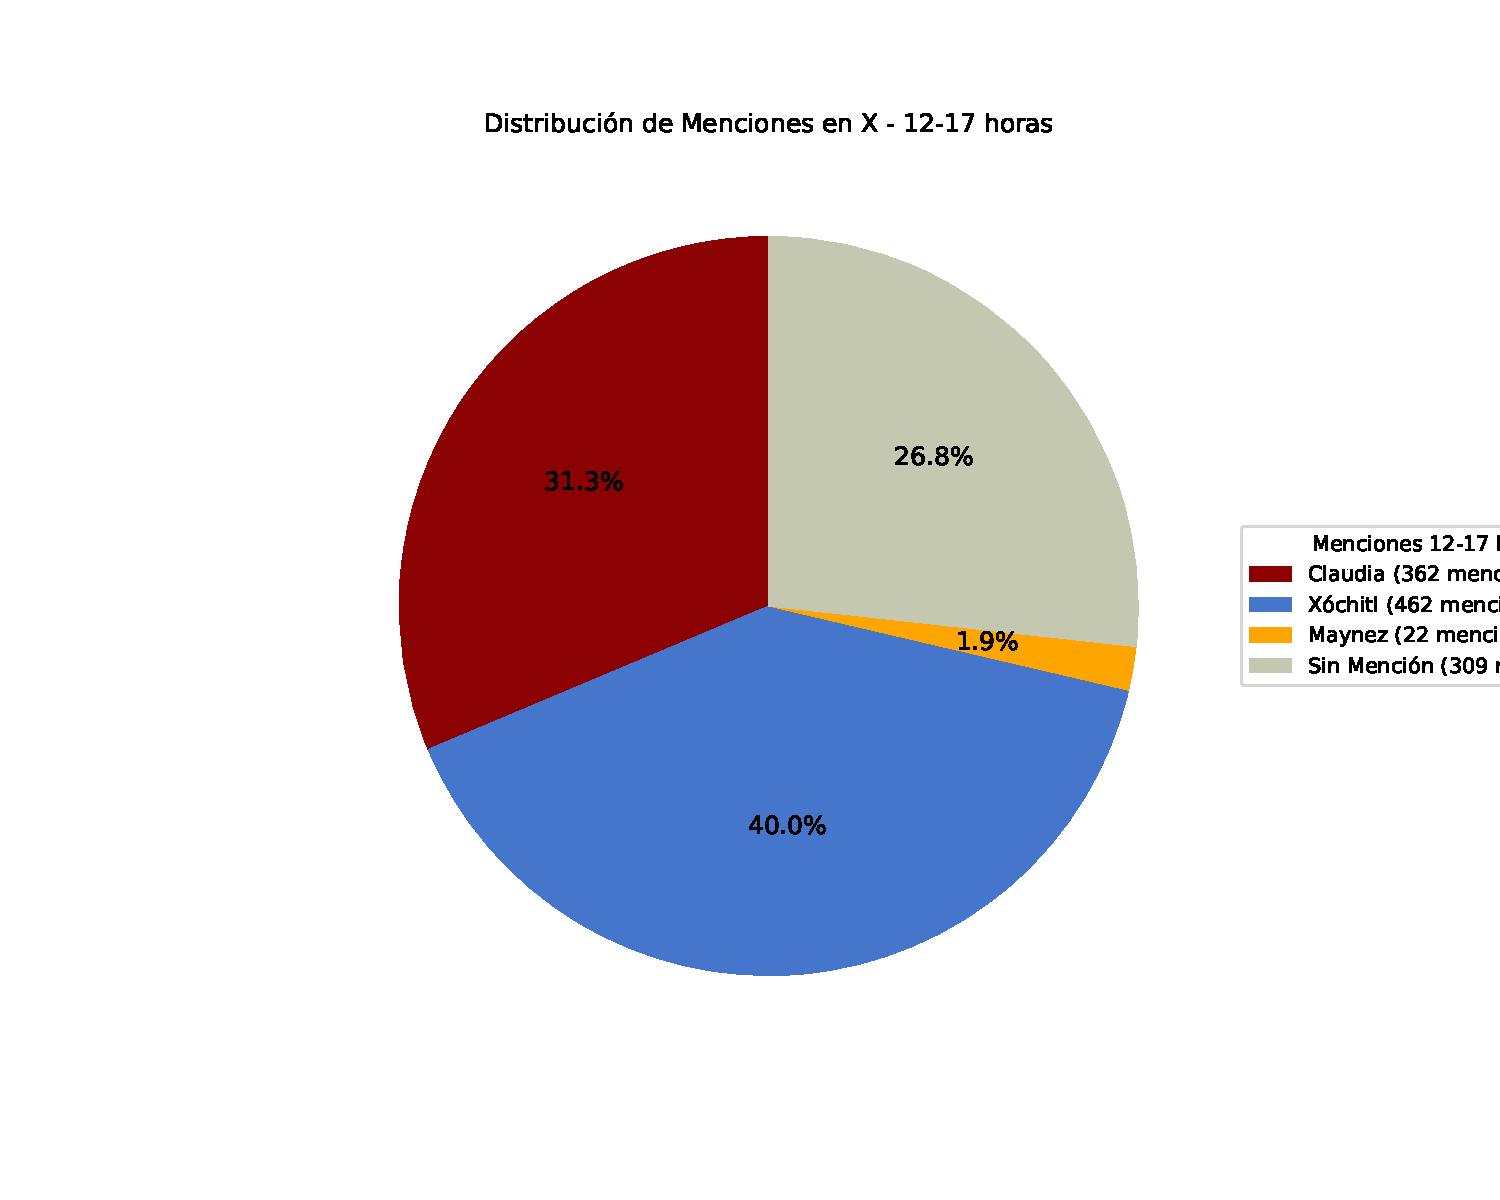
\includegraphics[width=\linewidth]{grafica_intervalo_12-17.pdf} 
			\vspace{-15mm}
			\caption{Distribución de Menciones de 12:00 a 17:00}
			\label{fig:xIntervalo1217}
		\end{minipage}
		\hfill % Espacio flexible entre las dos imágenes
		\begin{minipage}{0.49\textwidth}
			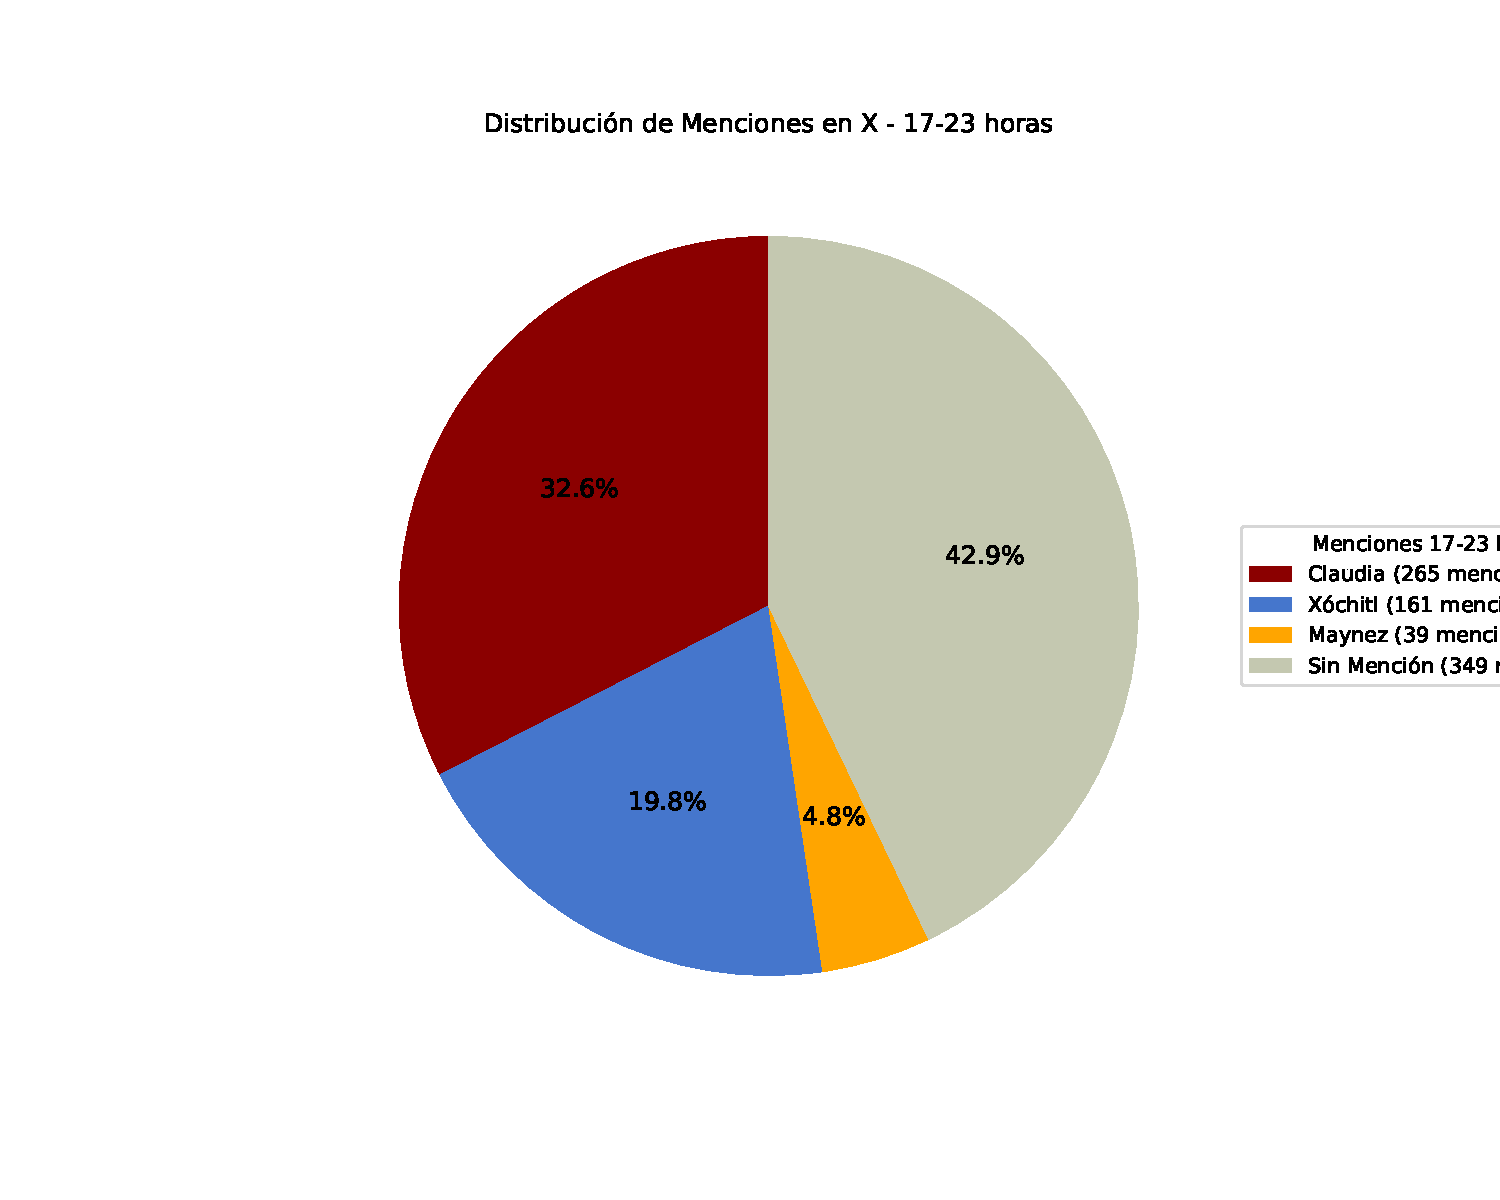
\includegraphics[width=\linewidth]{grafica_intervalo_17-23.pdf}
			\vspace{-15mm}
			\caption{Distribución de Menciones de 17:00 a 23:00}
			\label{fig:xIntervalo1723}
		\end{minipage}
	\end{figure}

	\begin{itemize}
		\item \textbf{Distribución Global:} La proporción de menciones entre Claudia Sheinbaum (32.9\%) y Xóchitl Gálvez (33.9\%) es muy similar, lo que refleja que ambas candidatas generaron un interés equiparable a nivel general. Jorge Álvarez Maynez, con solo el 2.8\% de las menciones, muestra una presencia muy limitada en las discusiones. Los comentarios sin mención específica representan un 30.4\%, lo que sugiere que una parte significativa de las publicaciones aborda temas generales del proceso electoral.
		
		\item \textbf{Intervalo 8-12 horas:} En las primeras horas del día, Xóchitl Gálvez domina con un 47.6\% de las menciones, mientras que Claudia Sheinbaum obtiene el 36.9\%. Jorge Álvarez Maynez tiene un 2.3\%, manteniendo su bajo nivel de atención. Solo el 13.1\% de las publicaciones no menciona candidatos, lo que indica que en este intervalo las discusiones estuvieron más focalizadas en los participantes.
		
		\item \textbf{Intervalo 12-17 horas:} Xóchitl Gálvez sigue liderando con un 39.1\%, aunque su ventaja frente a Claudia Sheinbaum (31.2\%) se reduce Jorge Álvarez Maynez continúa con un bajo porcentaje (1.7\%), lo que evidencia su falta de resonancia durante este intervalo. Las publicaciones sin mención específica aumentan al 27.9\%, lo que podría reflejar una mayor variedad de temas abordados por los usuarios.
		
		\item \textbf{Intervalo 17-23 horas:} Claudia Sheinbaum supera a Xóchitl Gálvez con un 32.7\% frente a 15.9\% de las menciones. Este cambio sugiere que hacia el cierre de la jornada electoral, Claudia captó más atención. Jorge Álvarez Maynez incrementa levemente su porcentaje a 4.6\%, aunque sigue siendo marginal. Las publicaciones sin mención específica alcanzan un 46.8\%, indicando un aumento significativo en los comentarios generales o no relacionados con los candidatos.
	\end{itemize}
	
	
	\subsubsection{Distribución Temporal}
	
	La distribución temporal es importante para identificar patrones y tendencias en la participación de los usuarios en diferentes momentos clave del proceso electoral. Este análisis permite observar cómo varía la cantidad de interacciones a lo largo del tiempo y cómo se concentran en fechas u horarios específicos. En este apartado se analiza la participación en los debates presidenciales y el comportamiento de los usuarios el día de la elección.
	
	\begin{figure}[h!]
		\centering
		\begin{minipage}{0.49\textwidth} % Mitad del ancho de la página
			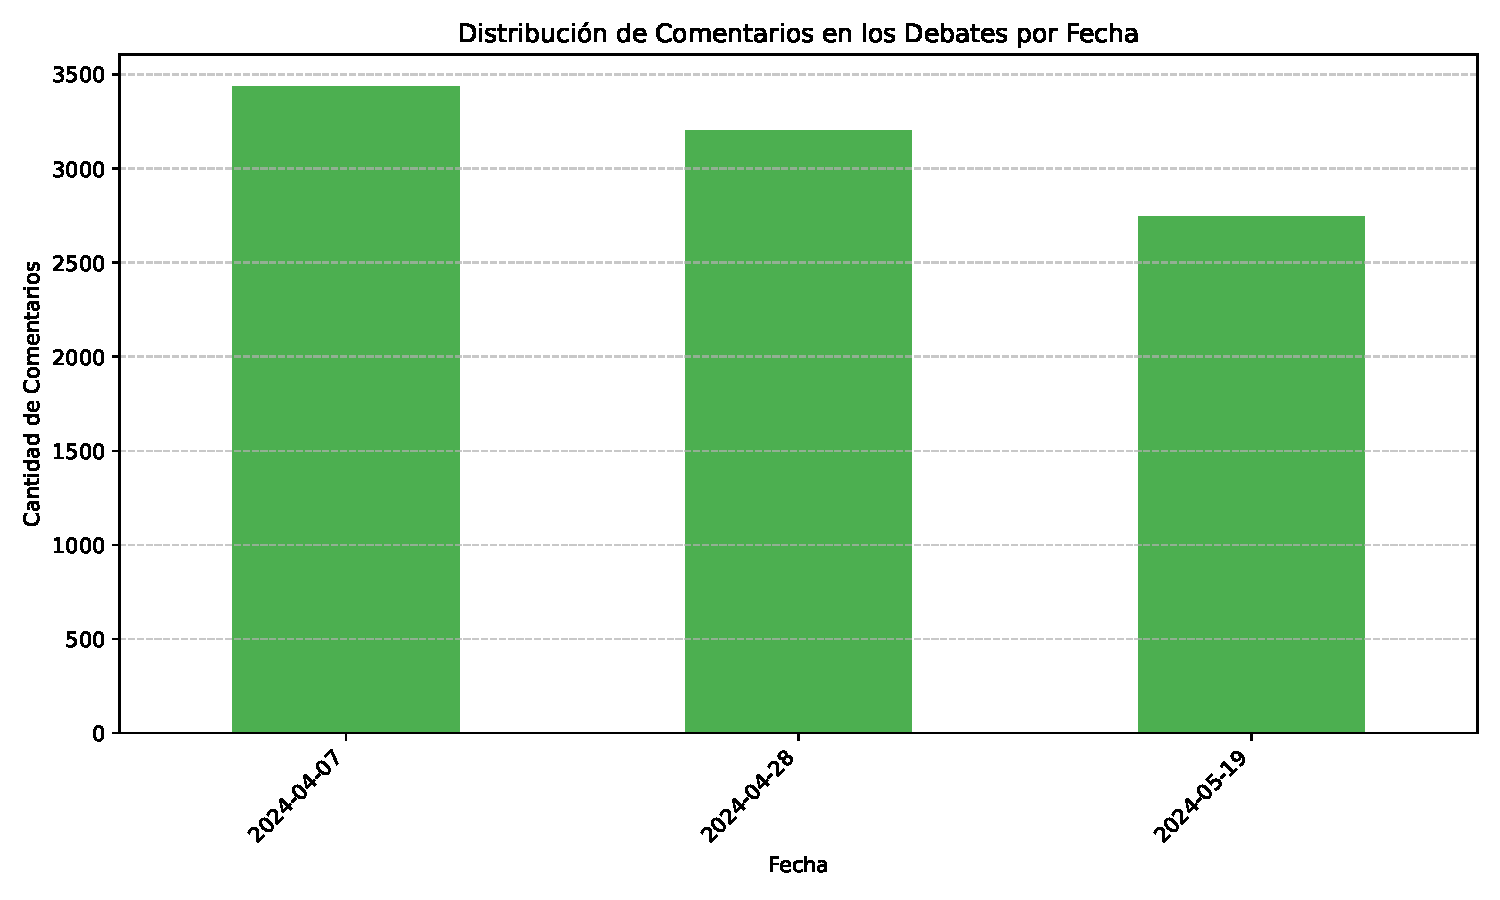
\includegraphics[width=\linewidth]{comentarios_fecha.pdf} 
			\vspace{-3mm}
			\caption{Distribución de Comentarios en los Debates por Fechas}
			\label{fig:temporalDebates}
		\end{minipage}
		\hfill % Espacio flexible entre las dos imágenes
		\begin{minipage}{0.49\textwidth}
			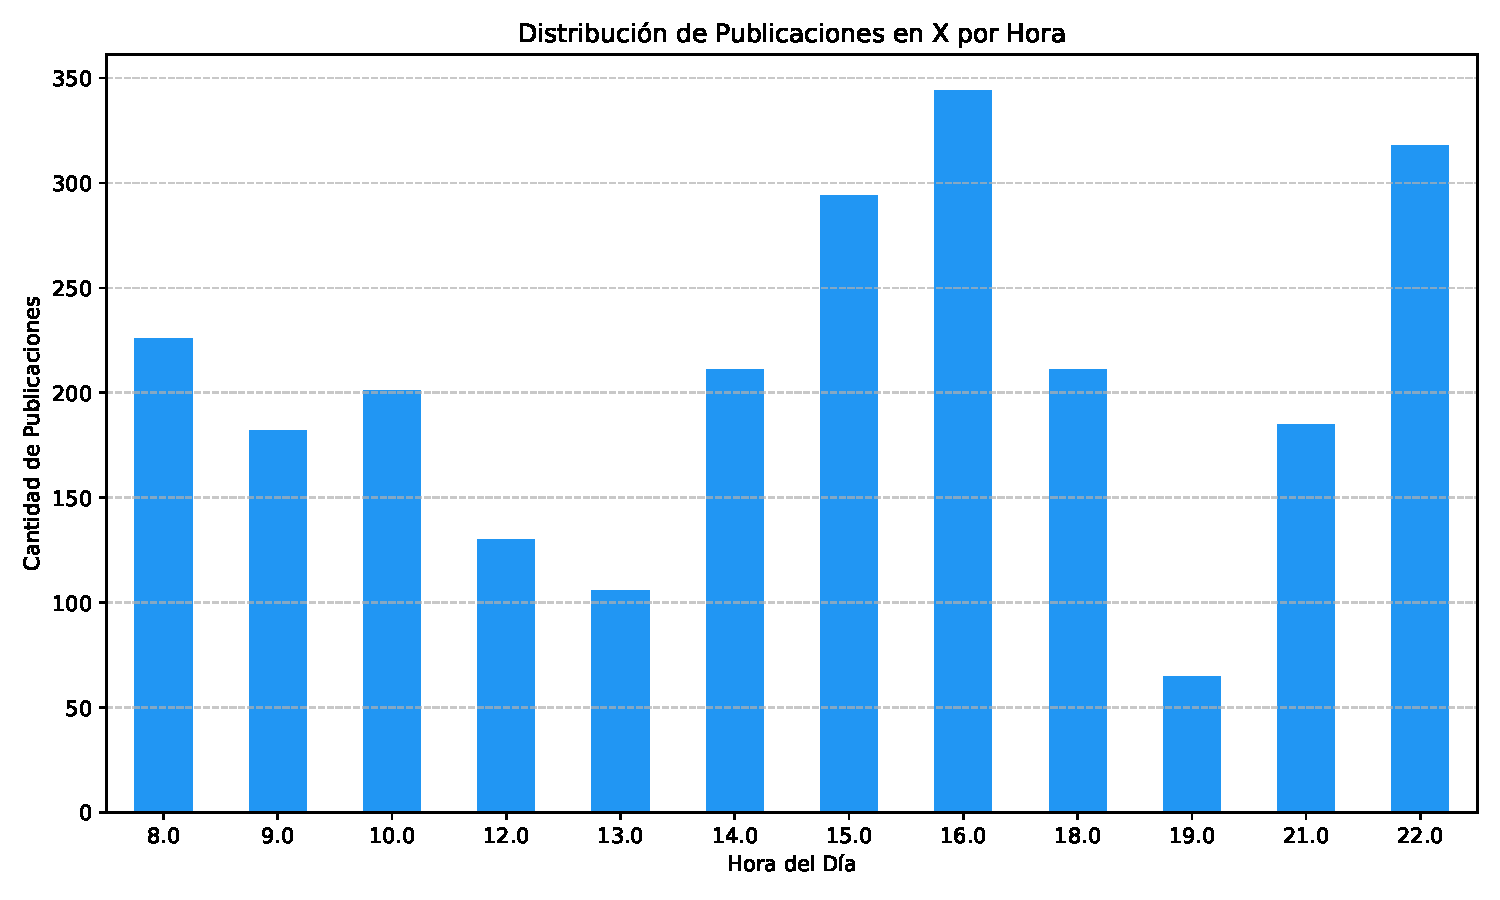
\includegraphics[width=\linewidth]{publicaciones_por_hora.pdf}
			\vspace{-3mm}
			\caption{Distribución de Comentarios en los Debates por Fechas}
			\label{fig:temporalDiaEleccion}
		\end{minipage}
	\end{figure}
	
	Como se muestra en la figura \ref{fig:temporalDebates}, la gráfica de distribución de comentarios en los debates muestra una participación constante a lo largo de los tres eventos. El debate del 7 de abril de 2024 tuvo el mayor número de comentarios, con un ligero descenso en los debates posteriores, especialmente en el del 19 de mayo de 2024. Esto podría indicar un alto interés inicial en las propuestas de los candidatos, que disminuyó ligeramente hacia el final del ciclo de debates, posiblemente debido a la repetición de ideas o al desgaste del público.
	
	Así también, se observa en la figura \ref{fig:temporalDiaEleccion} que la distribución de publicaciones por hora durante el día de la elección muestra picos claros de actividad a las 16:00 horas y nuevamente a las 22:00 horas, lo que podría reflejar el cierre de las casillas y las discusiones sobre los resultados preliminares. En contraste, las horas de la mañana (8:00-12:00) muestran una actividad moderada, probablemente relacionada con el inicio de la jornada electoral. El periodo de menor interacción ocurre alrededor de las 19:00 horas, lo que podría coincidir con un momento de pausa antes del cierre de las votaciones. Esto resalta cómo la actividad en redes sociales está vinculada a hitos clave del día electoral.
	
	
	\subsubsection{Análisis de frecuencias de palabras}
	
	En esta sección se realiza un análisis exploratorio para identificar las palabras más frecuentes en los comentarios y publicaciones relacionadas con los debates presidenciales y el día de la elección. Este análisis se lleva a cabo mediante la generación de nubes de palabras, que permiten visualizar de forma intuitiva los términos más recurrentes en los datos.
	
	\vspace{-4mm}
	\begin{figure}[h!]
		\centering
		\begin{minipage}{0.49\textwidth} % Mitad del ancho de la página
			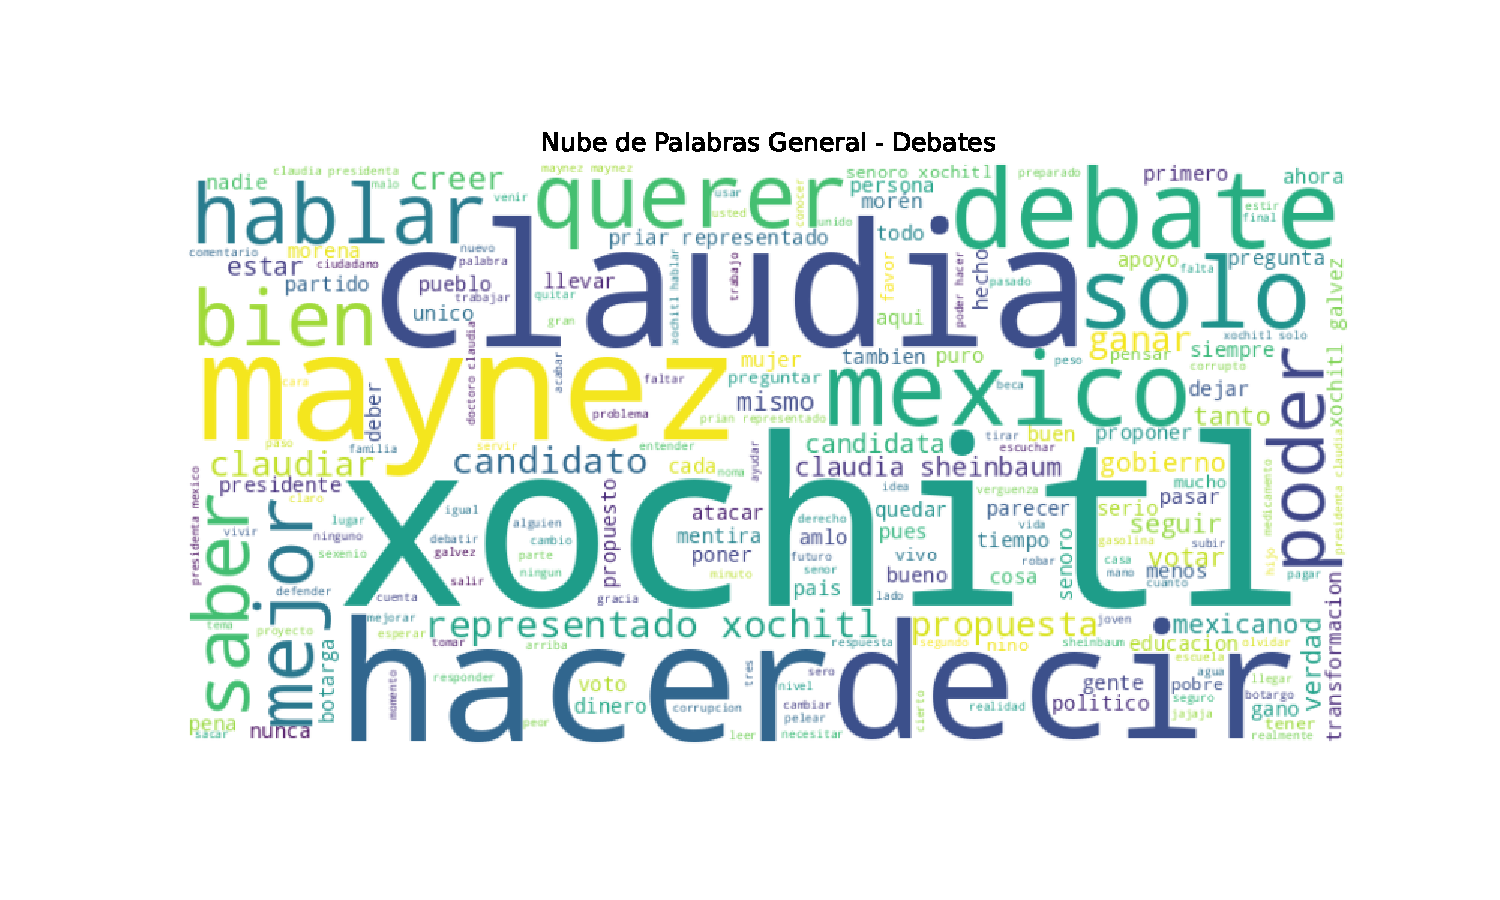
\includegraphics[width=\linewidth]{nube_palabras_general.pdf} 
			\vspace{-10mm}
			\caption{Distribución de Comentarios en los Debates por Fechas}
			\label{fig:Nube de Palabras de los Debates}
		\end{minipage}
		\hfill % Espacio flexible entre las dos imágenes
		\begin{minipage}{0.49\textwidth}
			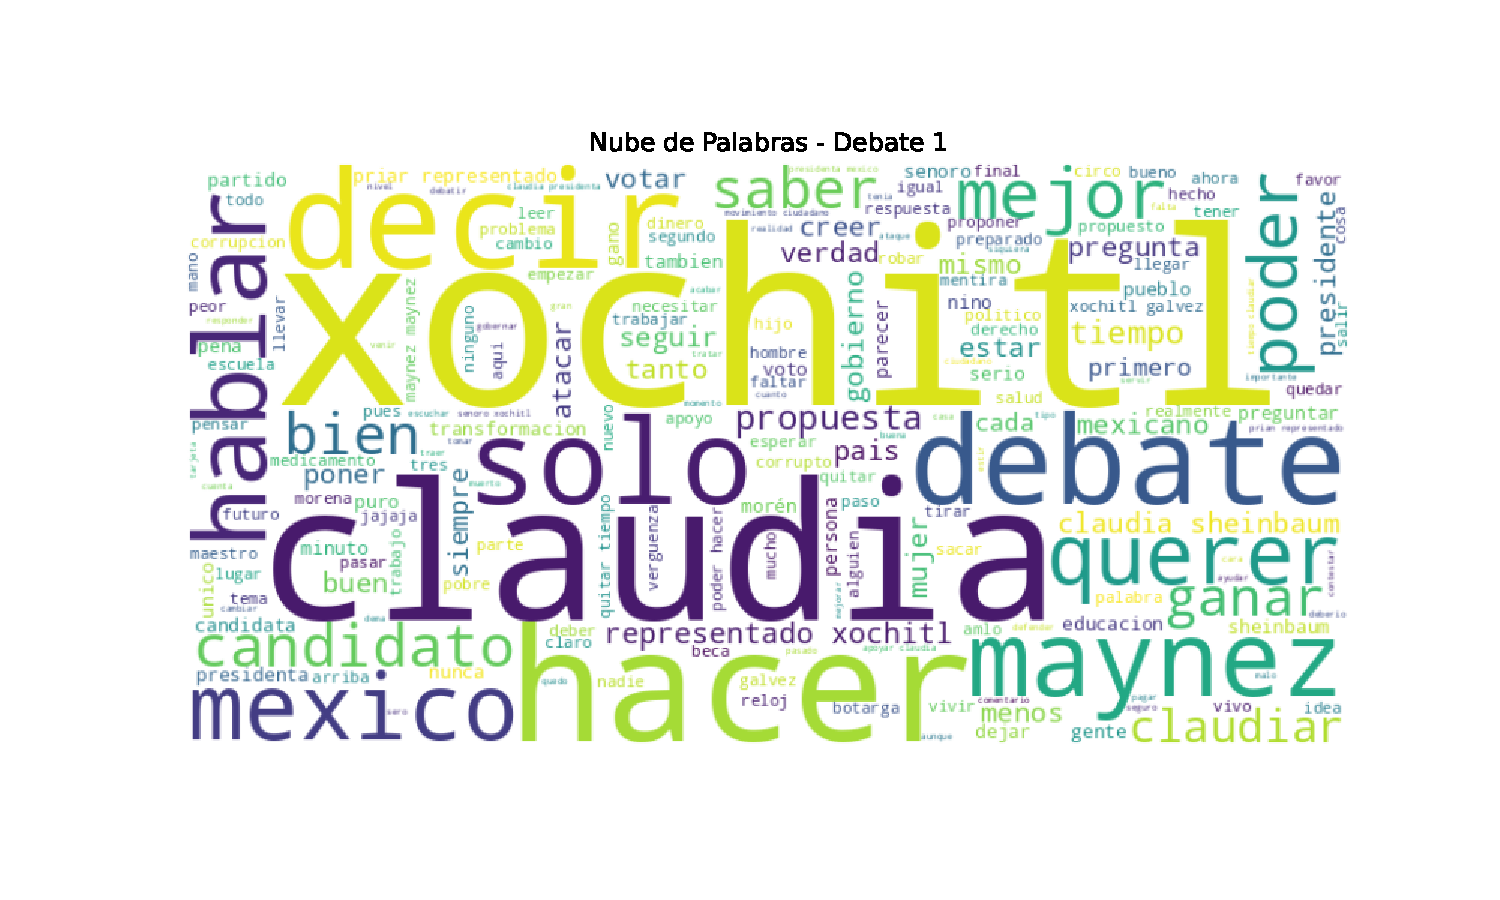
\includegraphics[width=\linewidth]{nube_palabras_debate_1.pdf}
			\vspace{-10mm}
			\caption{Nube de Palabras del Primer Debate}
			\label{fig:nubeDebate1}
		\end{minipage}
	\end{figure}
	
	
	\begin{figure}[h!]
		\centering
		\begin{minipage}{0.49\textwidth} % Mitad del ancho de la página
			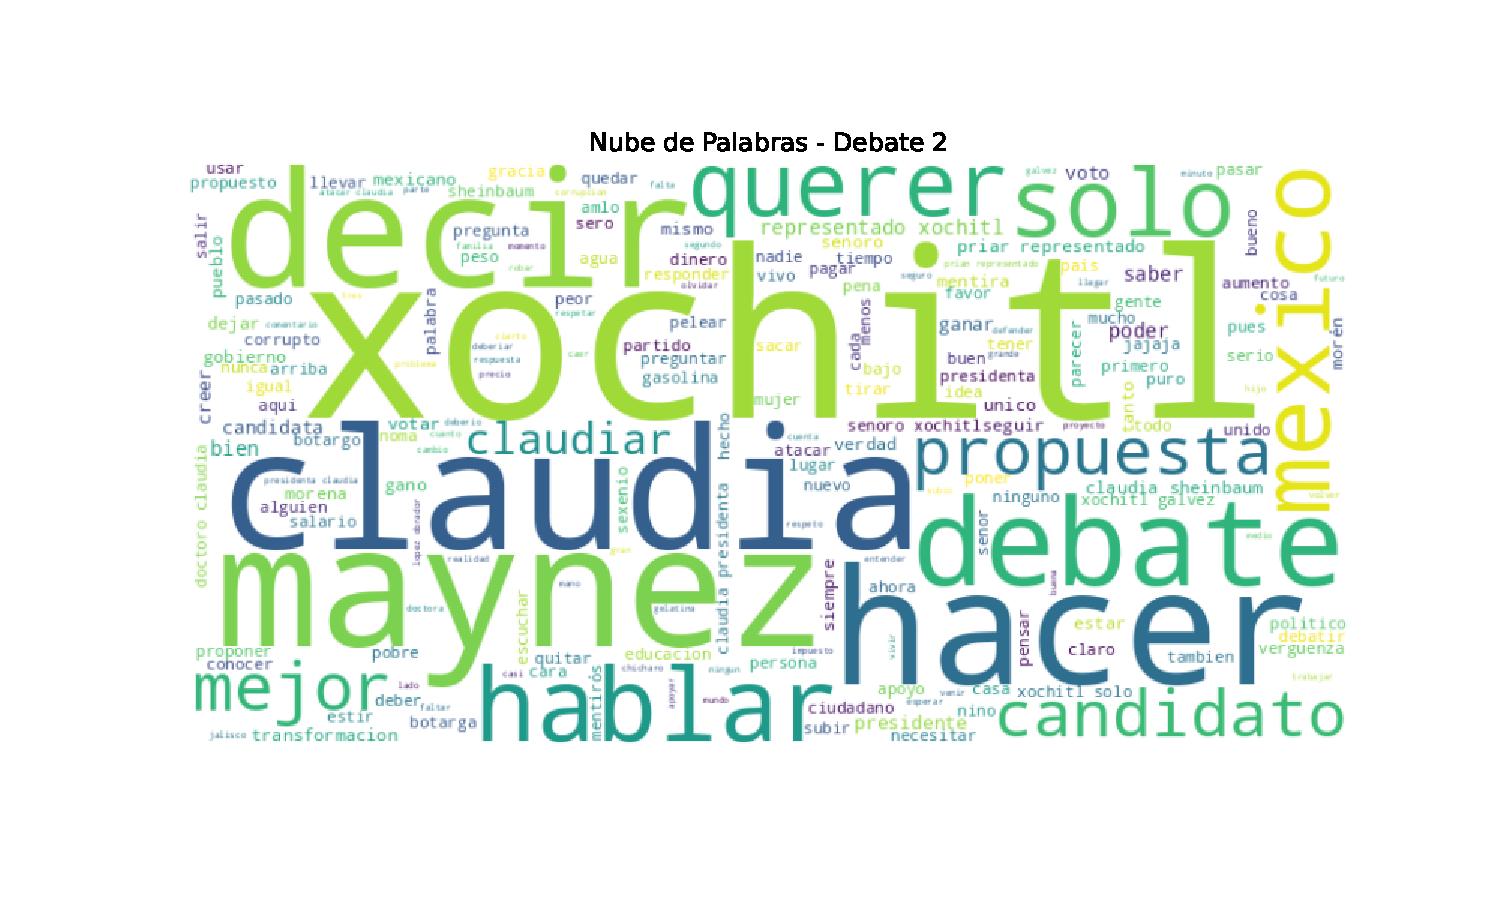
\includegraphics[width=\linewidth]{nube_palabras_debate_2.pdf} 
			\vspace{-10mm}
			\caption{Nube de Palabras del Segundo Debate}
			\label{fig:nubeDebate2}
		\end{minipage}
		\hfill % Espacio flexible entre las dos imágenes
		\begin{minipage}{0.49\textwidth}
			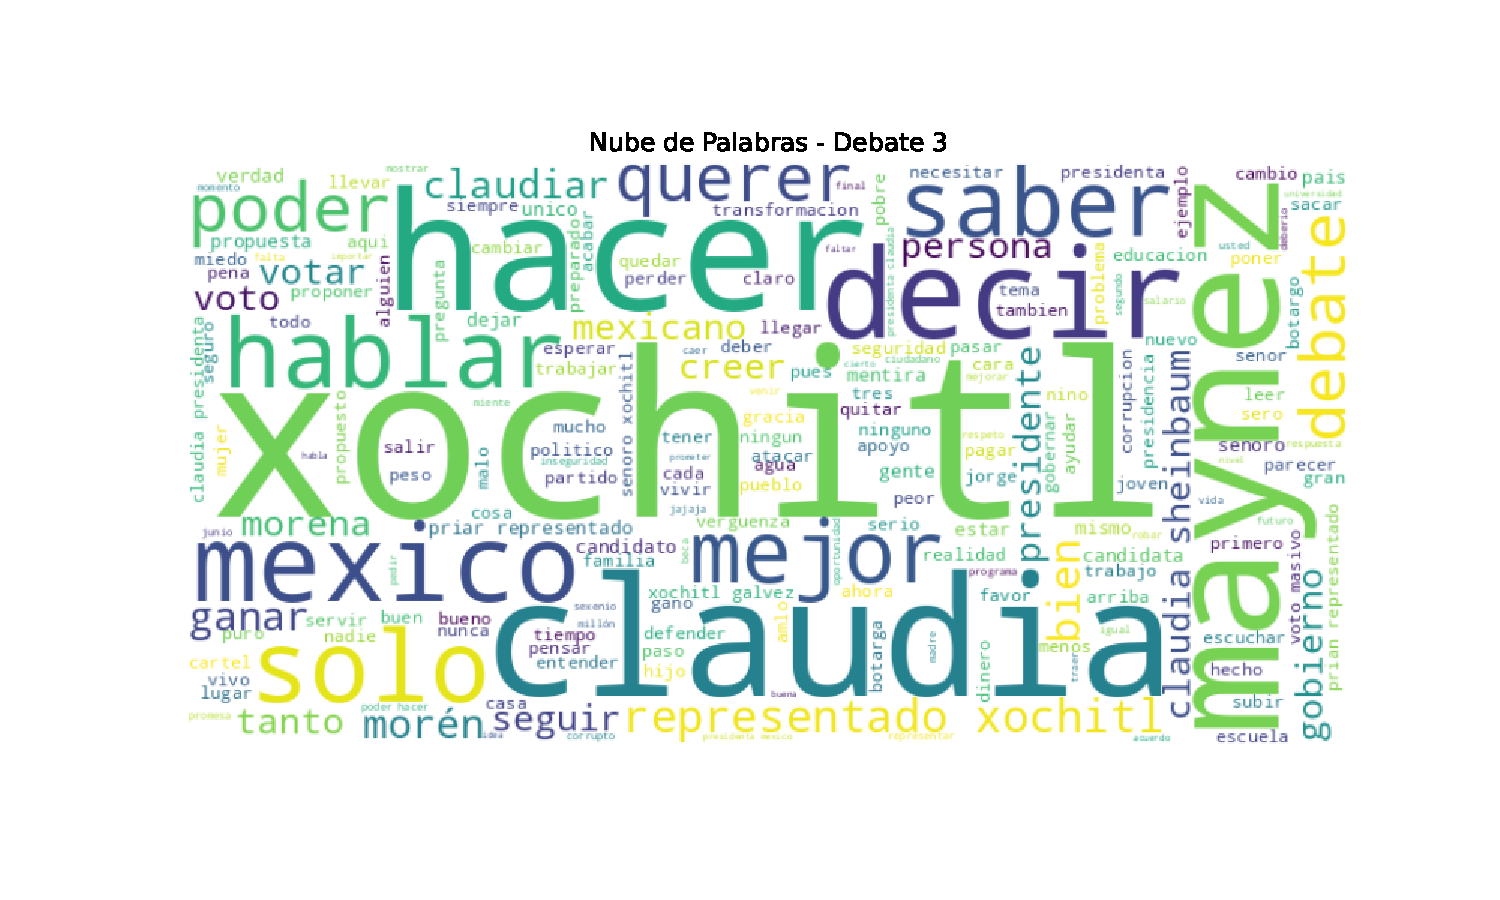
\includegraphics[width=\linewidth]{nube_palabras_debate_3.pdf}
			\vspace{-10mm}
			\caption{Nube de Palabras del Tercer Debate}
			\label{fig:nubeDebate3}
		\end{minipage}
	\end{figure}

	En la nube de palabras general de los debates, se observa una predominancia de términos como "decir", "hacer", "debate", "candidato" y menciones directas a los nombres de los candidatos, como "claudia", "xóchitl" y "maynez". Esto refleja que las discusiones se centran en las propuestas, el desempeño en los debates y las expectativas de los usuarios en torno a los participantes. Palabras relacionadas con el contexto político y social como "México", "gobierno" y "propuesta" también son frecuentes, indicando un interés en los temas tratados.
	
	Por otro lado, en las nubes de palabras individuales de los debates, se observan ligeras variaciones en los términos predominantes. Por ejemplo, en el primer debate destacan términos como "preguntar" y "atacar", lo que podría sugerir un enfoque más confrontativo. En el segundo debate, términos como "ganar" y "propuesta" son más prominentes, reflejando quizás un tono más propositivo. Finalmente, en el tercer debate, hay una recurrencia de términos como "hablar" y "decir", sugiriendo un interés en la claridad y el contenido de los mensajes. En conjunto, estas nubes reflejan cómo el enfoque y la percepción de los usuarios varían con el desarrollo de los debates.
	
	Replicando el mismo proceso para el día de la elección y considerando los intervalos definidos anteriormente, podemos observar las nubes descritas a continuación.
	
	\begin{figure}[h!]
		\centering
		\begin{minipage}{0.49\textwidth} % Mitad del ancho de la página
			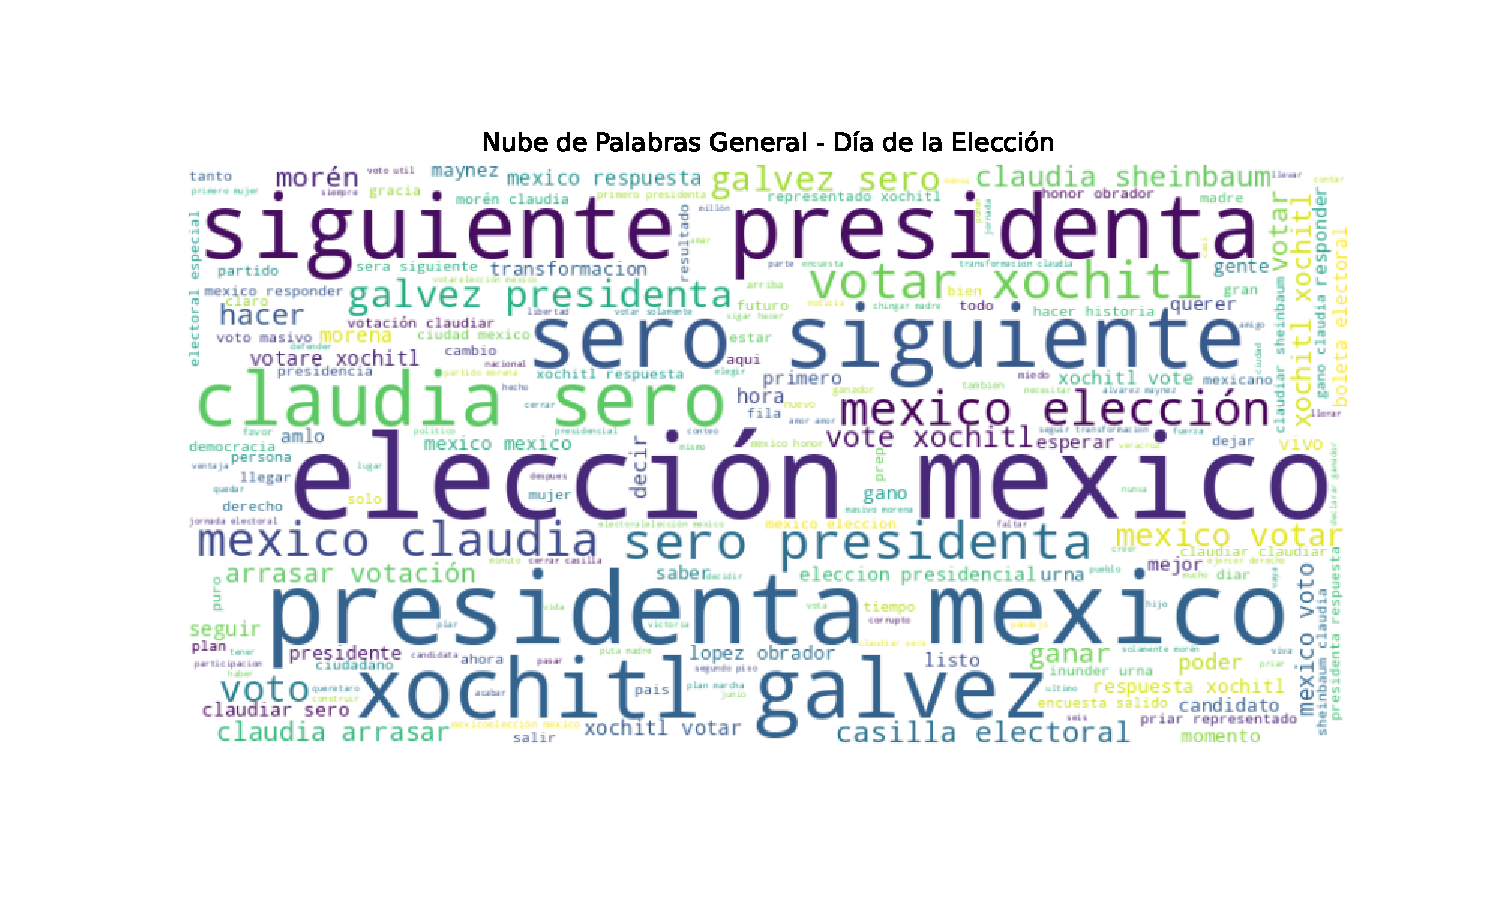
\includegraphics[width=\linewidth]{nube_general_eleccion.pdf} 
			\vspace{-10mm}
			\caption{Nube de Palabras del Día de la Elección}
			\label{fig:nubeDiaEleccion}
		\end{minipage}
		\hfill % Espacio flexible entre las dos imágenes
		\begin{minipage}{0.49\textwidth}
			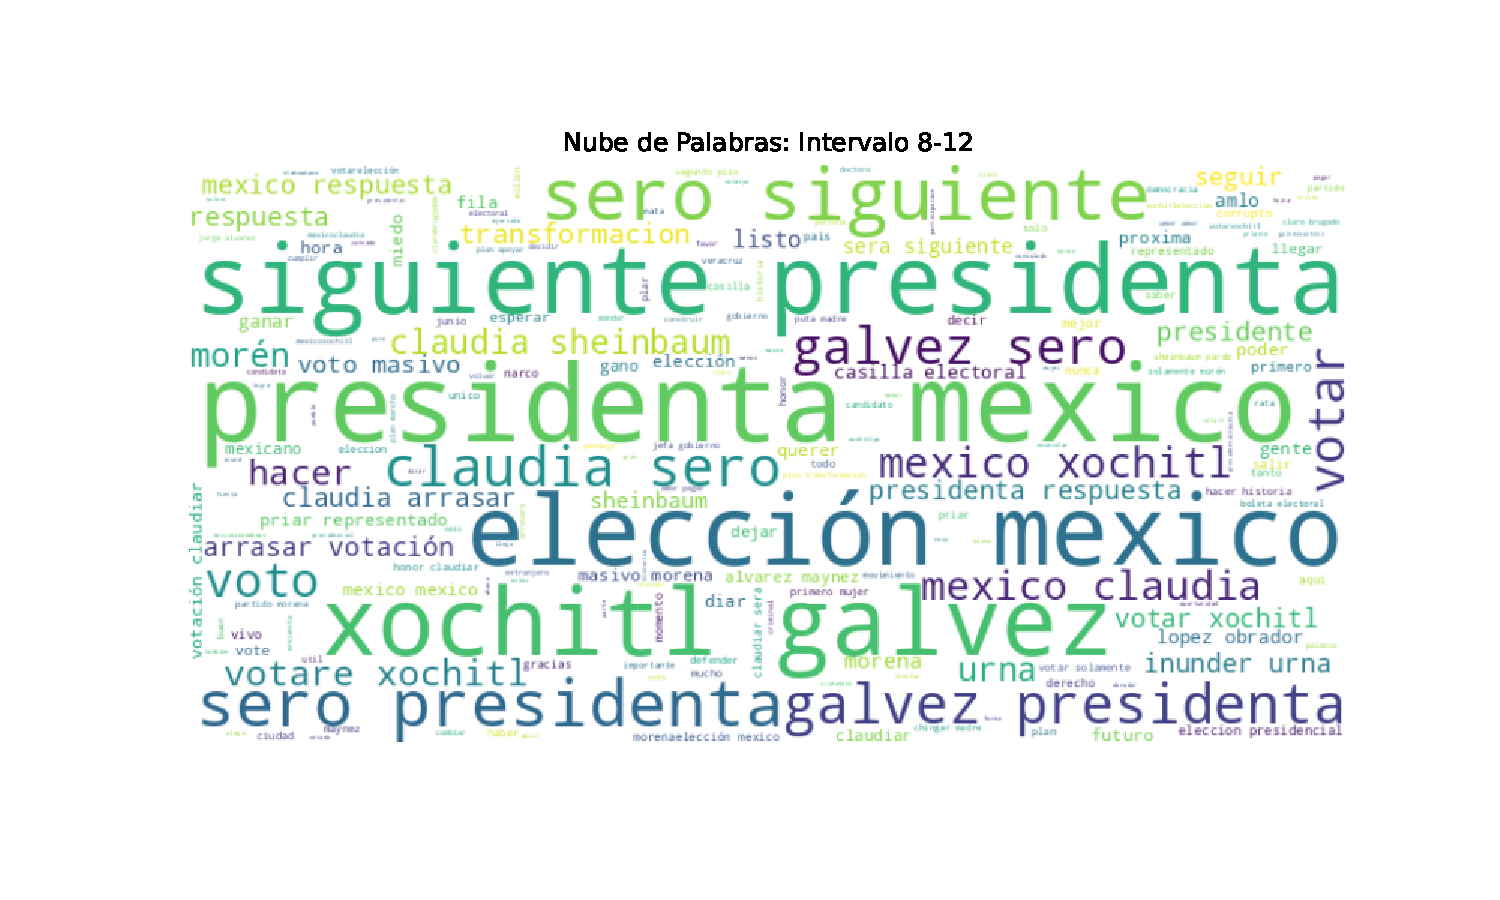
\includegraphics[width=\linewidth]{nube_intervalo_8-12.pdf}
			\vspace{-10mm}
			\caption{Nube de Palabras en el Horario de 08:00 a 12:00}
			\label{fig:nubeIntervalo812}
		\end{minipage}
	\end{figure}
	
	
	\begin{figure}[h!]
		\centering
		\begin{minipage}{0.49\textwidth} % Mitad del ancho de la página
			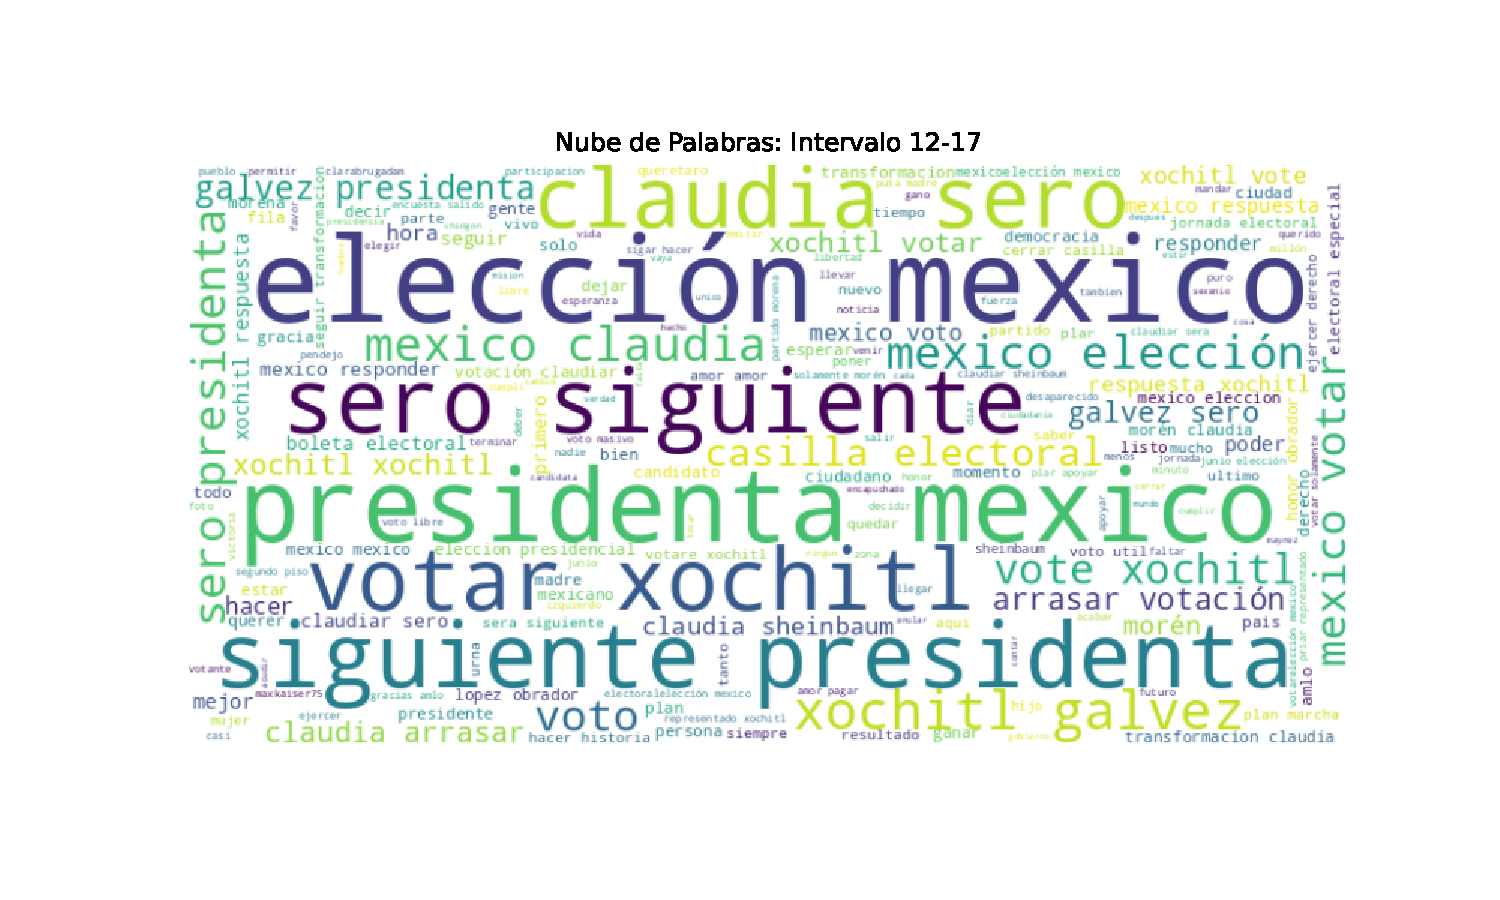
\includegraphics[width=\linewidth]{nube_intervalo_12-17.pdf} 
			\vspace{-10mm}
			\caption{Nube de Palabras en el Horario de 12:00 a 17:00}
			\label{fig:nubeIntervalo1217}
		\end{minipage}
		\hfill % Espacio flexible entre las dos imágenes
		\begin{minipage}{0.49\textwidth}
			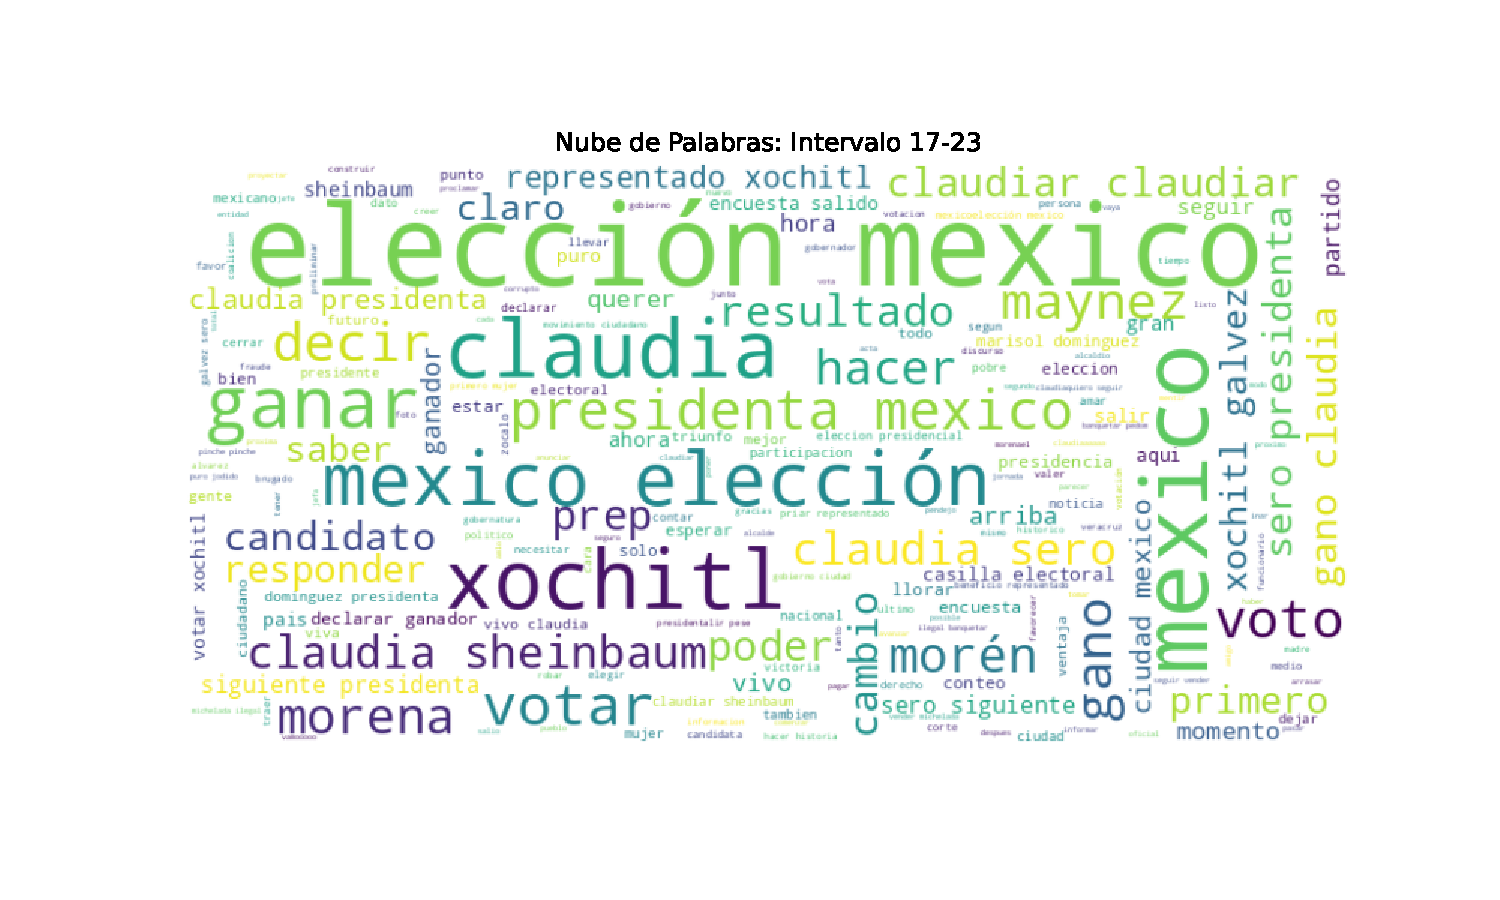
\includegraphics[width=\linewidth]{nube_intervalo_17-23.pdf}
			\vspace{-10mm}
			\caption{Nube de Palabras en el Horario de 08:00 a 12:00}
			\label{fig:nubeIntervalo1723}
		\end{minipage}
	\end{figure}

	En la nube general del día de la elección destaca términos como \textit{elección mexico}, \textit{votar}, \textit{siguiente presidenta}, \textit{xochitl galvez}. Esto refleja el enfoque de los usuarios en la jornada electoral, con énfasis en los principales candidatos y la participación ciudadana, indicando el interés por el proceso democrático.
	
	Y por intervalos, describimos a continuación las observaciones por cada uno:
	
	\begin{itemize}
		\item \textbf{Intervalo 8-12:} Las menciones predominantes incluyen términos como \textit{voto}, \textit{arrasar votación} y etiquetas relacionadas con ambos candidatos principales. Este periodo se caracteriza por mensajes incentivando el voto temprano y la participación.
		
		\item \textbf{Intervalo 12-17:} Se mantiene el protagonismo de \textit{votar xóchitl} y \textit{siguiente presidenta}, junto con menciones a \textit{casilla electoral}. Refleja el progreso del día y el aumento de interacciones relacionadas con el acto de votar.
		
		\item \textbf{Intervalo 17-23:} En las últimas horas, destacan términos como \textbf{ganar}, \textit{prep} y \textit{Claudia}. Esto indica una transición hacia la expectativa de resultados y comentarios finales sobre el cierre de casillas.
	\end{itemize}
	En general, las nubes reflejan cómo la narrativa cambia a lo largo del día, desde promover la participación hasta debatir resultados y candidatos clave.
	
	
	\subsubsection{Análisis de Engagement (YouTube)}
	
	En esta sección se analiza el nivel de interacción que generan los comentarios en los debates presidenciales, utilizando como indicador principal el número de "me gusta" (num\_likes). Este análisis busca identificar patrones asociados a los comentarios más populares, como su relación con la longitud del texto, el contenido o el debate en el que fueron realizados. Asimismo, se revisan los comentarios con más "likes" para comprender las opiniones y temas que generaron mayor resonancia entre los usuarios.
	
	\begin{table}[H]
		\centering
		\begin{tabular}{|c|p{11cm}|c|c|}
			\hline
			\textbf{ID} & \textbf{Comentario} & \textbf{Num Likes} & \textbf{Num Debate} \\ \hline
			3831 & Es en serio lo que dijo la candidata Xochitl. ¿Pregúntenle a los muertos?. Que tonterías dice y sin razón. & 823 & 1 \\ \hline
			3848 & Imagínense que Xochitl quedara de presidente. No mms la peor vergüenza mundial que nos podría pasar & 745 & 1 \\ \hline
		\end{tabular}
		\caption{Ejemplo de comentarios relacionados con Xóchitl Gálvez, con sus respectivos likes y debate.}
		\label{tab:comentarios_xochitl}
	\end{table}
	
	\begin{table}[H]
		\centering
		\begin{tabular}{|c|p{11cm}|c|c|}
			\hline
			\textbf{ID} & \textbf{Comentario} & \textbf{Num Likes} & \textbf{Num Debate} \\ \hline
			3832 & Xochitl galvez es un peña nieto cualquiera & 717 & 1 \\ \hline
			3839 & Xóchitl se pone nerviosa en un debate y se traba al expresarse. Imagínate para dirigir un país & 661 & 1 \\ \hline
			2529 & Bla bla bla. A estas alturas. Ya sabemos quién miente. No somos pendejos. & 545 & 3 \\ \hline
		\end{tabular}
		\caption{Ejemplo de comentarios relacionados con Xóchitl Gálvez, con sus respectivos likes y debate.}
		\label{tab:comentarios_xochitl2}
	\end{table}
	
	Observaciones sobre los comentarios más populares
	
	Los comentarios con mayor número de "me gusta" tienden a centrarse en juicios hacia los candidatos, utilizando un tono crítico y humorístico. En particular, los cinco comentarios más populares observados tienen en común:
	
	\begin{itemize}
		\item \textbf{Foco en Xóchitl Gálvez:} Todos los comentarios hacen referencia directa a Xóchitl, lo que sugiere que su participación en los debates generó un alto nivel de interacción.
		\item \textbf{Tono crítico o sarcástico:} Los usuarios tienden a usar ironías o críticas contundentes, que parecen captar más atención y \textit{me gusta}.
		\item \textbf{Debate predominante:} Cuatro de los cinco comentarios están relacionados con el primer debate, lo que indica que este evento pudo haber generado el mayor nivel de controversia y participación.
	\end{itemize}
	
	
	\subsubsection{Análisis de Longitud y Complejidad de Comentarios}
	En esta sección se evalúa la longitud de los comentarios en YouTube y las publicaciones en la plataforma X, medida en cantidad de palabras. Este análisis permite comprender la complejidad y nivel de detalle de las interacciones en ambas plataformas. Se utiliza la longitud promedio como un indicador clave y se visualiza mediante histogramas que muestran la distribución de la frecuencia de palabras. Además, una línea punteada roja señala el promedio, ayudando a identificar si los comentarios suelen ser más extensos o concisos. Este enfoque facilita detectar patrones relacionados con la profundidad de las opiniones de los usuarios.
	
	\begin{figure}[h!]
		\centering
		\begin{minipage}{0.49\textwidth} % Mitad del ancho de la página
			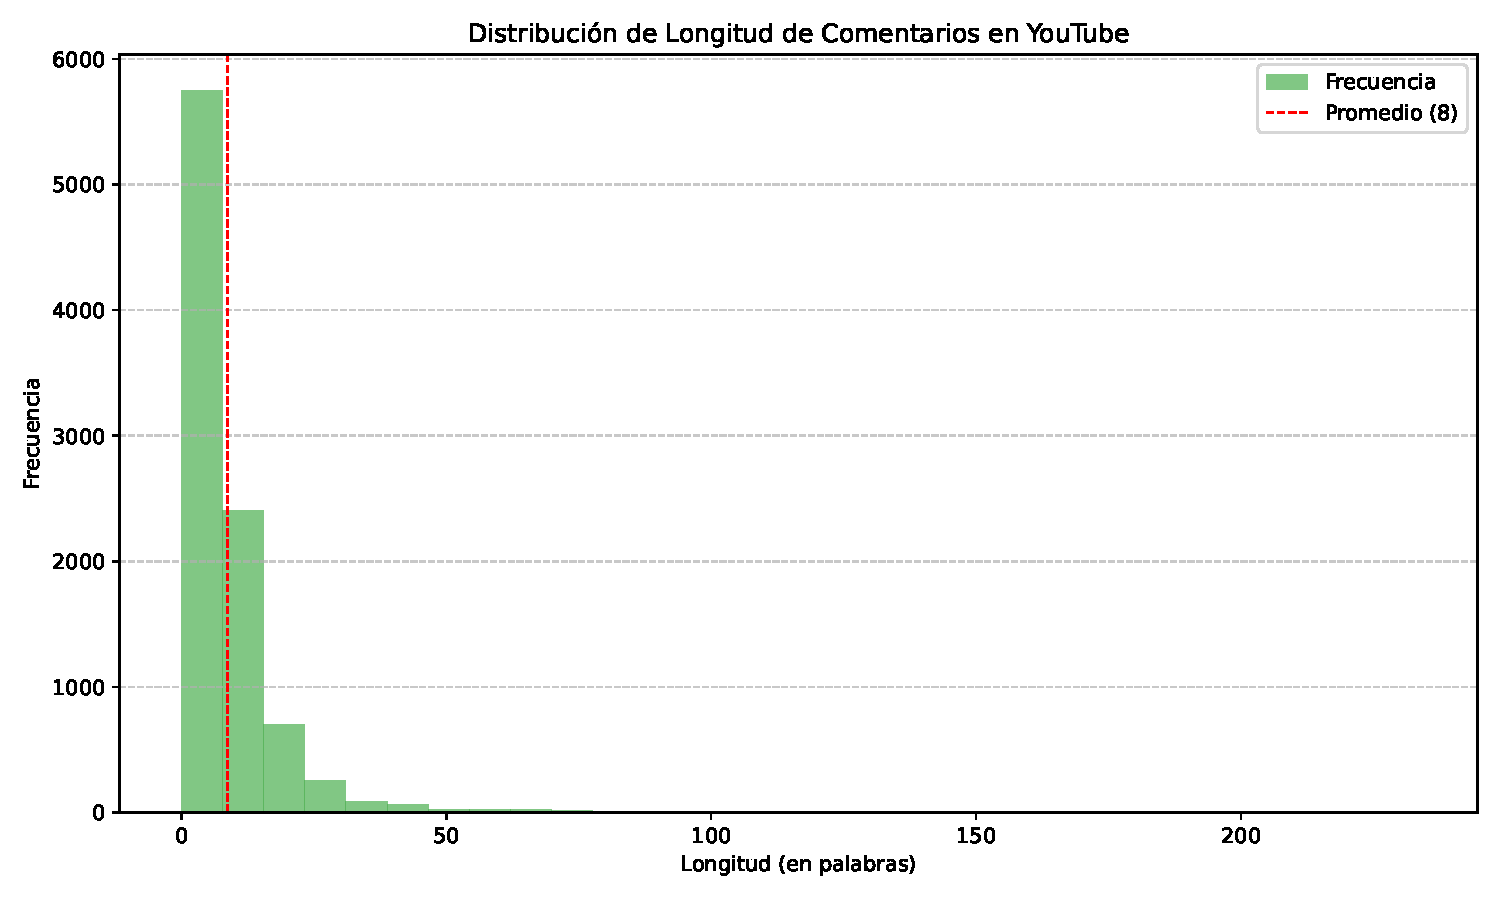
\includegraphics[width=\linewidth]{longitud_comentarios_youtube.pdf} 
			\vspace{-2mm}
			\caption{Distribución de Longitud de Comentarios en Youtube}
			\label{fig:longYoutube}
		\end{minipage}
		\hfill % Espacio flexible entre las dos imágenes
		\begin{minipage}{0.49\textwidth}
			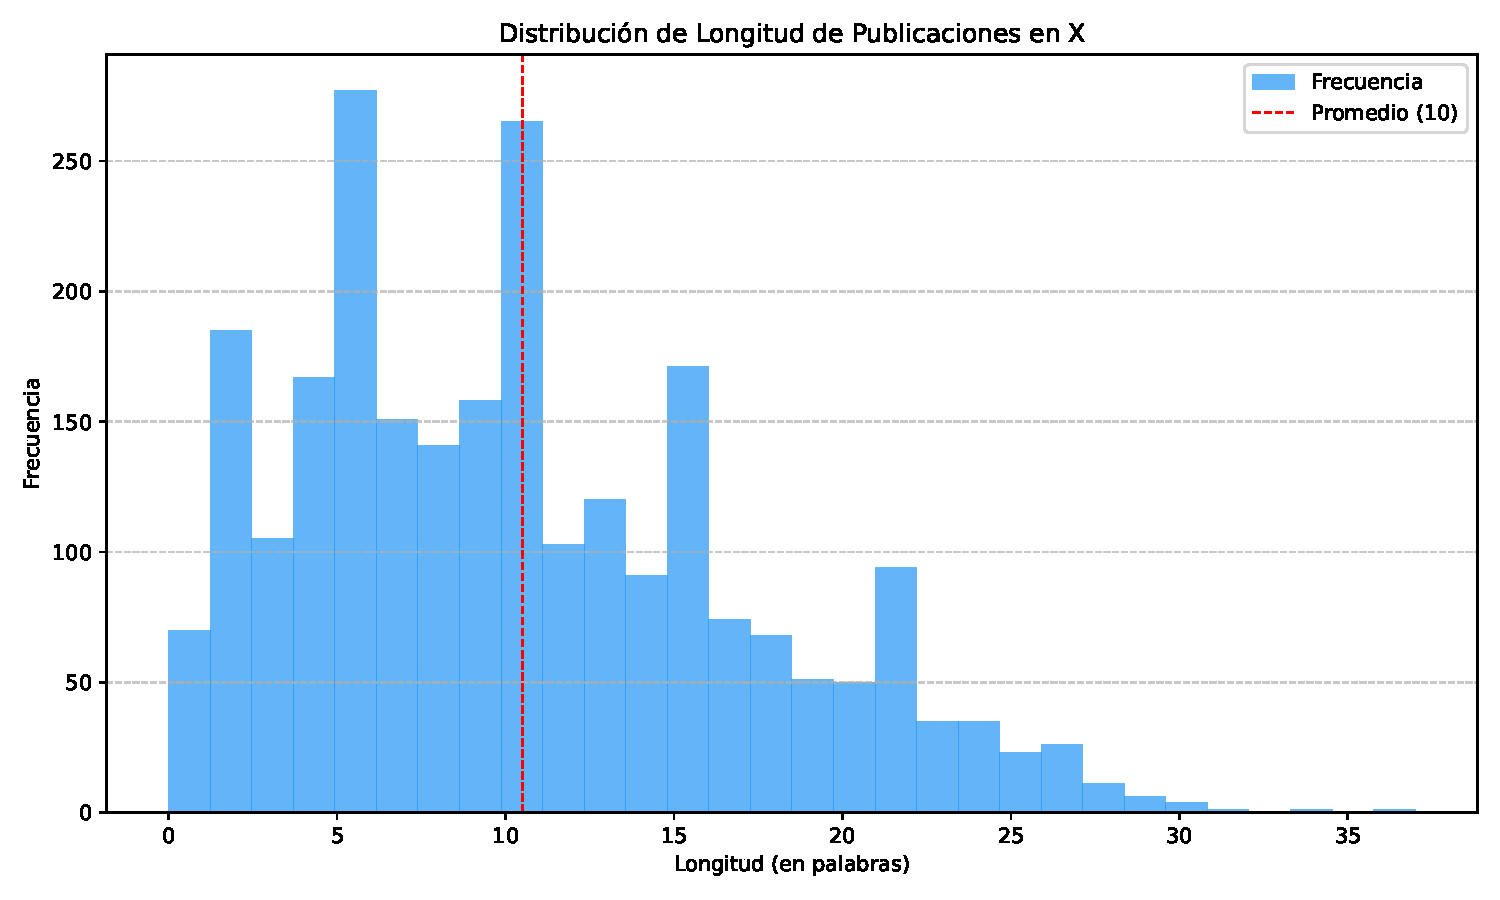
\includegraphics[width=\linewidth]{longitud_publicaciones_x.pdf}
			\vspace{-2mm}
			\caption{Distribución de Longitud de Publicaciones en X}
			\label{fig:longX}
		\end{minipage}
	\end{figure}
	
	
	En los histogramas presentados se observa la distribución de la longitud de los comentarios y publicaciones en los datasets de YouTube (figura \ref{fig:longYoutube}) y X (figura \ref{fig:longX}), respectivamente.
	
	\begin{enumerate}
		\item \textbf{YouTube:} La mayoría de los comentarios tienen una longitud muy corta, con un promedio de 8 palabras. Esto indica que los usuarios en esta plataforma tienden a realizar aportaciones concisas, posiblemente debido a la naturaleza del contenido de YouTube, que fomenta interacciones rápidas y directas. Sin embargo, hay una pequeña cantidad de comentarios que alcanzan longitudes mayores, reflejando una profundidad ocasional en el discurso.
		
		\item \textbf{X:} Las publicaciones en X también muestran un comportamiento de longitud predominantemente corto, con un promedio ligeramente menor, de 10 palabras. Esto puede atribuirse al formato de la plataforma, históricamente restringido en caracteres, lo que impulsa a los usuarios a ser breves. Sin embargo, se observa una mayor variabilidad en las longitudes en comparación con YouTube, con publicaciones que alcanzan hasta más de 30 palabras, posiblemente reflejando usuarios aprovechando la extensión actualizada de caracteres.
	\end{enumerate}
	
	\subsubsection{Conclusiones Preliminares}
	\textbf{De la Participación por Fecha y Plataforma:} En YouTube, la mayor cantidad de comentarios se concentra en el primer debate, disminuyendo ligeramente en los debates posteriores. Esto sugiere que el interés disminuyó conforme avanzaron los debates. En X, las publicaciones se distribuyen de manera más uniforme a lo largo del día de la elección, con un pico notable en los intervalos de la tarde, entre las 12:00 y 17:00, indicando una mayor actividad cuando se reportan resultados preliminares o momentos clave.
	
	\textbf{De las Menciones a Candidatos:} En ambos datasets, Claudia Sheinbaum y Xóchitl Gálvez presentan una proporción similar de menciones, reflejando su protagonismo en la conversación electoral. Jorge Álvarez Maynez tiene una participación significativamente menor.Un alto porcentaje de comentarios no menciona explícitamente a ningún candidato, lo que puede implicar discusiones generales sobre los debates o temas relacionados con la elección sin una referencia directa a los candidatos.
	
	\textbf{De la Frecuencia de Palabras:} En las nubes de palabras de los debates, los términos más frecuentes están relacionados con "decir", "hacer", "propuestas" y los nombres de los candidatos, reflejando un enfoque en las declaraciones y promesas durante los debates. En el día de la elección, destacan palabras como "eleccionesmexico2024", "votar", "casilla" y "resultados", lo que subraya la interacción centrada en el acto de votar y la espera de resultados.
	
	\textbf{Del Engagement (YouTube):} Los comentarios con mayor número de likes tienden a ser más críticos o emocionales, especialmente hacia ciertos candidatos, lo que sugiere que las opiniones polarizadas generan mayor interacción.
	
	\textbf{De la Longitud y Complejidad:} Los comentarios en YouTube tienen un promedio de 8 palabras, mientras que las publicaciones en X tienen un promedio de 7 palabras, reflejando la naturaleza breve y directa de las interacciones en ambas plataformas. En ambas plataformas, la distribución de longitud es altamente sesgada hacia comentarios muy cortos, con pocas interacciones más elaboradas.
	
	\textbf{\textit{Resumen General}}
	
	Los resultados reflejan patrones importantes de participación y discurso en redes sociales durante el contexto electoral. Los candidatos principales, Claudia Sheinbaum y Xóchitl Gálvez, dominan la conversación, mientras que Jorge Álvarez Maynez tiene un impacto menor. Las palabras clave destacan el enfoque de los usuarios en propuestas y resultados, mientras que las interacciones tienden a ser breves y rápidas, acorde al formato de las plataformas.
	
	\subsection{Análisis de Sentimientos}
	Para analizar las opiniones expresadas en los comentarios y publicaciones de las redes sociales, se desarrolló un proceso de etiquetado de datos diseñado específicamente para capturar los matices del sentimiento en un contexto electoral multietiqueta. Este proceso consideró que un comentario puede expresar sentimientos hacia más de un candidato y, por tanto, el conjunto de datos se configuró para admitir múltiples etiquetas asociadas a un solo registro.
	
	\subsubsection{Codificación de Sentimientos}
	
	Se adoptó una codificación consistente para representar los sentimientos asociados a los candidatos principales de las elecciones presidenciales de México 2024, incluyendo un cuarto candidato virtual denominado \textit{Ninguno}. Este último se empleó en los casos donde los comentarios o publicaciones no hacían referencia explícita a ninguno de los candidatos reales. Las etiquetas se asignaron de la siguiente manera:
	
	\begin{itemize}
		\item \textbf{-1:} Sentimiento negativo hacia un candidato.
		\item \textbf{0:} Sentimiento neutral o ausencia de mención hacia el candidato en cuestión.
		\item \textbf{1:} Sentimiento positivo hacia un candidato.
	\end{itemize}
	
	Los candidatos considerados en el etiquetado fueron:
	\begin{itemize}
		\item \textbf{Claudia Sheinbaum}
		\item \textbf{Xóchitl Gálvez}
		\item \textbf{Jorge Álvarez Maynez}
		\item \textbf{Ninguno} (candidato virtual)
	\end{itemize}
	
	
	Se establecieron lineamientos específicos para garantizar que las etiquetas reflejaran de manera precisa los sentimientos y opiniones expresados en los comentarios. Las principales consideraciones fueron las siguientes:
	
	\begin{enumerate}
		\item \textbf{Críticas al gobierno actual:} Se etiquetaron como sentimientos negativos hacia Claudia Sheinbaum, dado su vínculo con el partido en el poder.
		\item \textbf{Descalificaciones generales:} Comentarios como ``no hay ni a quién irle'' se etiquetaron con sentimiento negativo hacia los tres candidatos.
		\item \textbf{Críticas específicas a propuestas o lemas:} Cuando un comentario hacía referencia a una propuesta o lema de campaña, se marcó el sentimiento hacia el candidato que lo propuso.
		\item \textbf{Críticas a partidos o coaliciones:} En este caso, el sentimiento se asoció al candidato representante del partido o coalición mencionada.
		\item \textbf{Uso de apodos:} Se tuvo en cuenta el uso consistente de apodos en los comentarios para asociar el sentimiento con el candidato correspondiente.
	\end{enumerate}
	
	
	Se desarrolló una herramienta específica para facilitar este proceso, permitiendo asignar etiquetas a los comentarios de forma manual y precisa. La herramienta fue diseñada para soportar múltiples etiquetas por comentario, siguiendo la estructura multietiqueta del conjunto de datos. A continuación, se incluye una imagen que ilustra la interfaz y funcionalidad de esta herramienta:
	
	\begin{figure}[H]
		\centering
		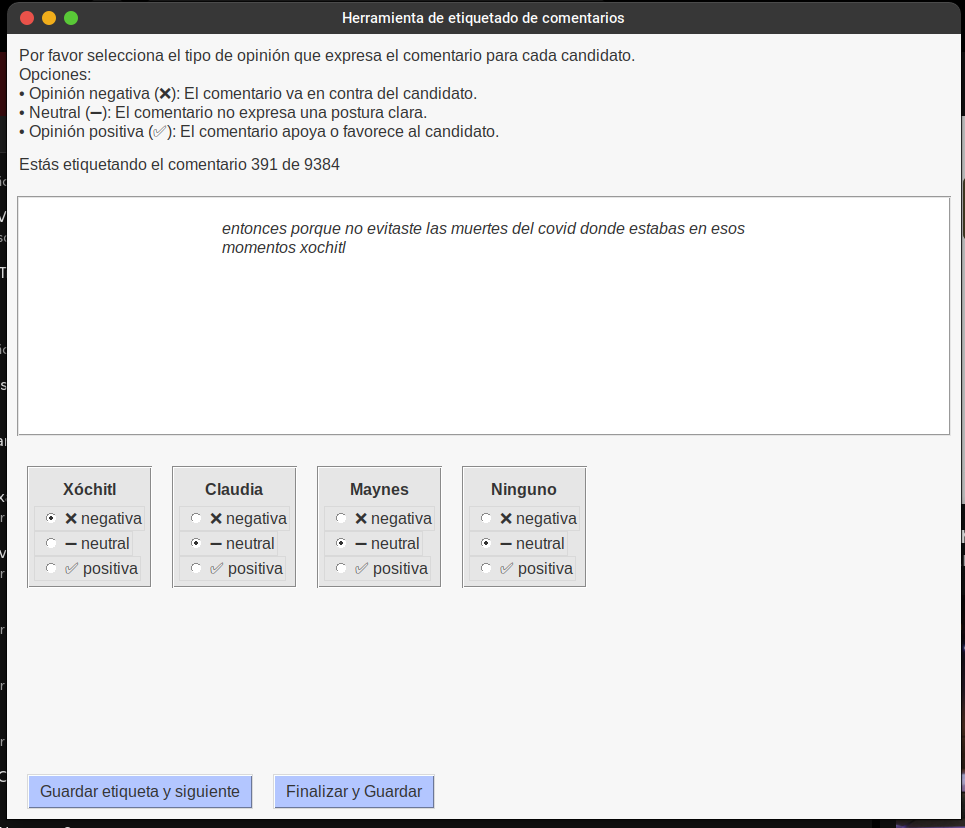
\includegraphics[width=0.6\textwidth]{etiquetado.png}
		\caption{Interfaz de la herramienta de etiquetado desarrollada para el análisis de sentimiento.}
		\label{fig:etiquetado}
	\end{figure}
	
	Esta herramienta fue de utilidad para garantizar la consistencia en el proceso de etiquetado, permitiendo que los datos reflejen los patrones de opinión expresados por los usuarios en YouTube y X.
	
	Como resultado del proceso de etiquetado descrito, se obtuvieron dos conjuntos de datos en formato tabular, el primero consta de 4,000 datos etiquetados correspondientes a los debates presidenciales, y el segundo con 1,000 datos etiquetados tomados de manera aleatoria del dia de la elección. Dichos datasets contienen las siguientes columnas adicionales:
	
	\begin{itemize}
		\item \texttt{Claudia:} Sentimiento expresado hacia Claudia Sheinbaum.
		\item \texttt{Maynez:} Sentimiento expresado hacia Jorge Álvarez Maynez.
		\item \texttt{Ninguno:} Sentimiento expresado hacia ningún candidato real.
		\item \texttt{Xóchitl:} Sentimiento expresado hacia Xóchitl Gálvez.
	\end{itemize}
	
	
	
	\subsubsection{BETO Fine-Tuning}
	
	Para la clasificación de sentimientos en los comentarios recopilados sobre los debates y el día de la elección, se realizó un proceso de fine-tuning del modelo pre-entrenado BETO (\textit{BERT en español}). Este modelo se adaptó para comprender el contexto político y la jerga mexicana relacionada con la jornada electoral de México 2024, permitiendo etiquetar automáticamente el resto de los comentarios no procesados manualmente.
	
	En primer lugar, para que el modelo de inteligencia pudiera entender mejor las etiquetas, se realizó una recodificación de los sentimientos:
	\begin{itemize}
		\item \(-1 \rightarrow 0\) (sentimiento negativo),
		\item \(0 \rightarrow 1\) (sentimiento neutral),
		\item \(1 \rightarrow 2\) (sentimiento positivo).
	\end{itemize}

	
	Se combinaron los dos conjuntos de datos (comentarios de debates y comentarios del día de la elección) en un único dataset con las siguientes columnas:
	\begin{itemize}
		\item \texttt{comentario\_editado}: Texto del comentario.
		\item \texttt{Claudia}, \texttt{Xóchitl}, \texttt{Maynez}, \texttt{Ninguno}: Etiquetas de sentimiento asociadas a cada candidato.
	\end{itemize}
	
	El problema se definió como una clasificación multietiqueta de tres clases (positivo, neutral y negativo) asociadas a cuatro categorías (los candidatos y la categoría ``Ninguno''). Esto resulta en un total de 12 clases (\(3 \times 4\)).
	
	Para combatir el desequilibrio en las clases, se realizaron los siguientes pasos:
	\begin{itemize}
		\item \textbf{Undersampling}: Se eliminaron 250 registros con etiquetas que indicaban sentimientos neutrales para los tres candidatos principales (\texttt{Xóchitl = 1, Claudia = 1, Maynez = 1}), buscando reducir el ruido en los datos.
		\item \textbf{Pesos de Clase}: Se utilizó la técnica \texttt{compute\_class\_weight} para calcular los pesos de clase, que luego fueron incorporados en una variante de la función de pérdida \texttt{CrossEntropyLoss}.
	\end{itemize}
	
	Propiamente hablando, el modelo fine-tuned incluyó los siguientes elementos:
	\begin{itemize}
		\item \textbf{BETO Pre-entrenado}: Se usó el token \texttt{[CLS]} como el vector de características representativo del significado global del comentario.
		\item \textbf{Clasificador Tipo MLP}: Se diseñó un perceptrón multicapa (MLP) cuya salida consistió en 12 logits:
		\begin{itemize}
			\item Logits \(0-2\): Sentimientos hacia Xóchitl.
			\item Logits \(3-5\): Sentimientos hacia Claudia.
			\item Logits \(6-8\): Sentimientos hacia Maynez.
			\item Logits \(9-11\): Sentimientos hacia Ninguno.
		\end{itemize}
		Para cada grupo de 3 logits se aplicó una función \texttt{softmax}, garantizando que las probabilidades en cada grupo sumen 1.
	\end{itemize}
	
	Dicho modelo se entrenó utilizando los siguientes parámetros: \(16\) en el tamaño del batch y \(3\) épocas de fine-tuning. 
	
	Con ello, el modelo fine-tuned logró un accuracy general del \textbf{81.3\%}, destacándose especialmente en la clasificación de sentimientos hacia \textbf{Xóchitl} con un 83.8\% de precisión, seguida de \textbf{Claudia} con un 81.2\% y \textbf{Maynez} con un 78.9\%. Las matrices de confusión revelan que el modelo clasificó correctamente la mayoría de los ejemplos neutrales, aunque los sentimientos negativos tendieron a confundirse con neutrales en algunos casos.
	
	\begin{figure}[h!]
		\centering
		\begin{minipage}{0.4\textwidth} % Mitad del ancho de la página
			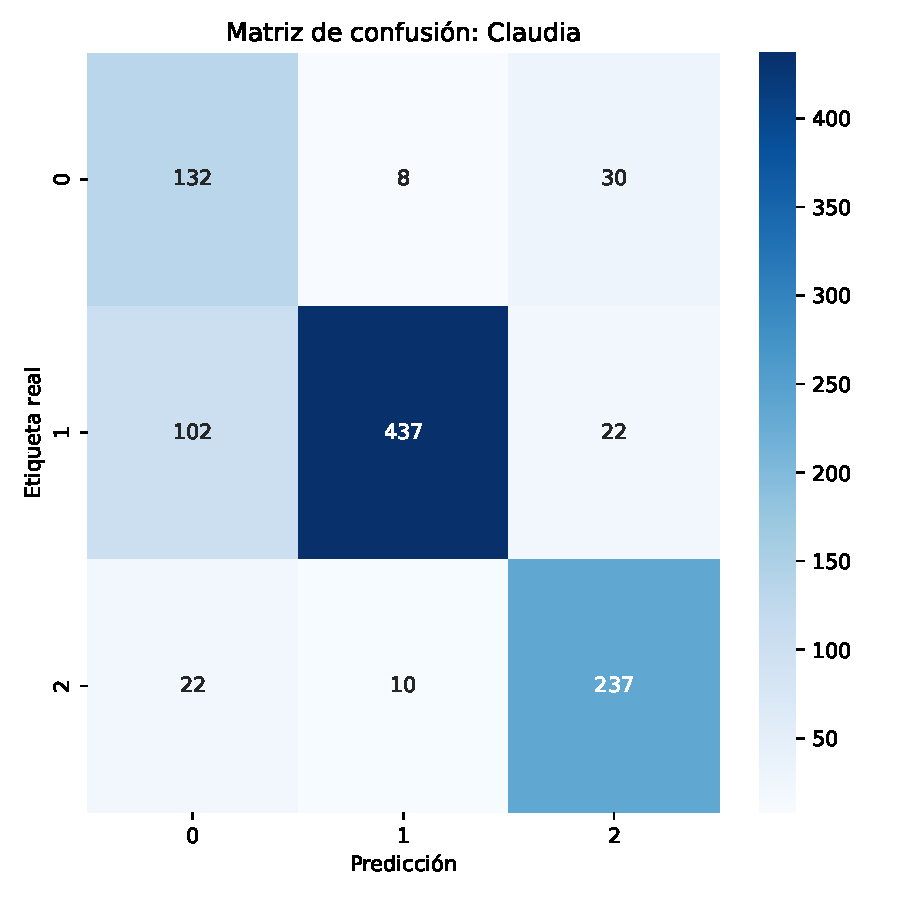
\includegraphics[width=\linewidth]{conf_matrix_Claudia.pdf} 
			\caption{Matriz de confusión para Claudia.}
			\label{fig:cmClaudia}
		\end{minipage}
		\hfill % Espacio flexible entre las dos imágenes
		\begin{minipage}{0.4\textwidth}
			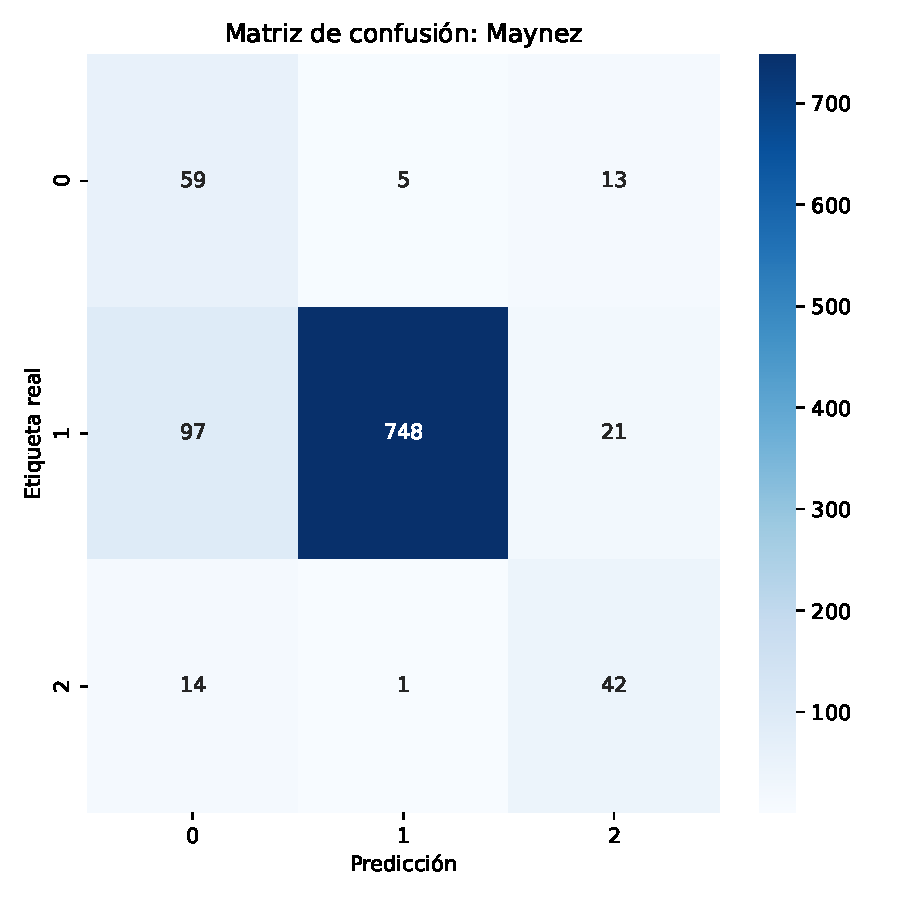
\includegraphics[width=\linewidth]{conf_matrix_Maynez.pdf}
			\caption{Matriz de confusión para Maynez.}
			\label{fig:cmMaynez}
		\end{minipage}
	\end{figure}
	
	\begin{figure}[h!]
		\centering
		\begin{minipage}{0.4\textwidth} % Mitad del ancho de la página
			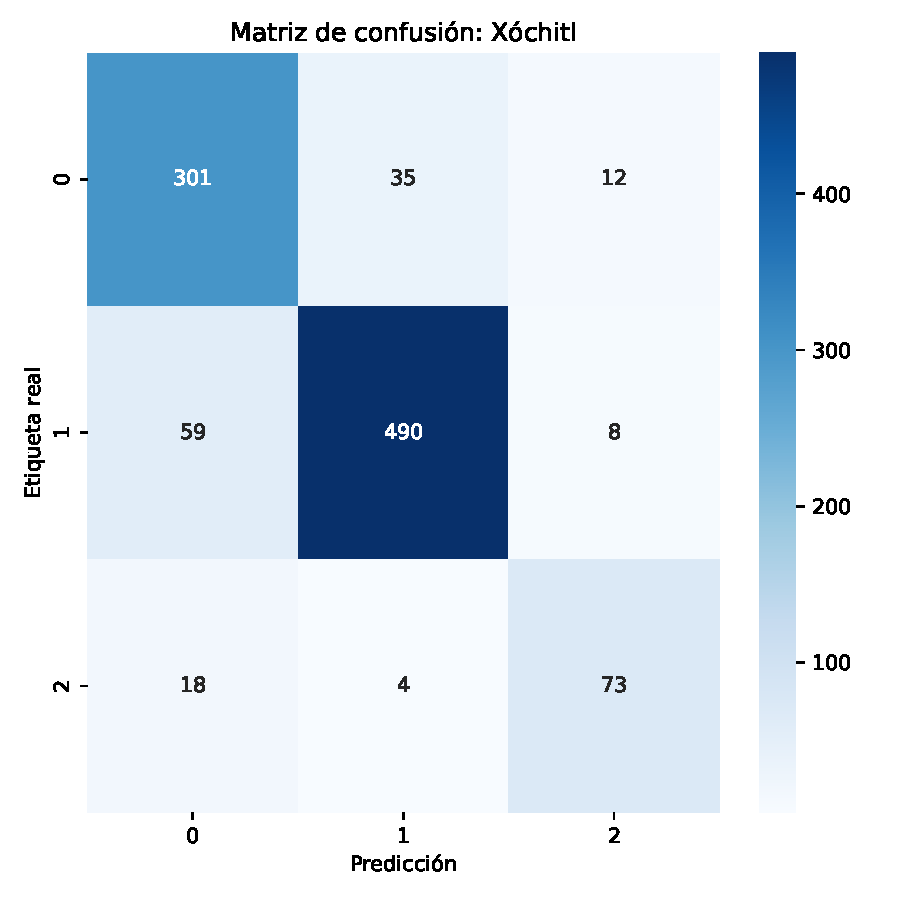
\includegraphics[width=\linewidth]{conf_matrix_Xóchitl.pdf} 
			\caption{Matriz de confusión para Xóchitl.}
			\label{fig:cmXochitl}
		\end{minipage}
	\end{figure}

	\vspace{-3mm}
	\begin{figure}[H]
		\centering
		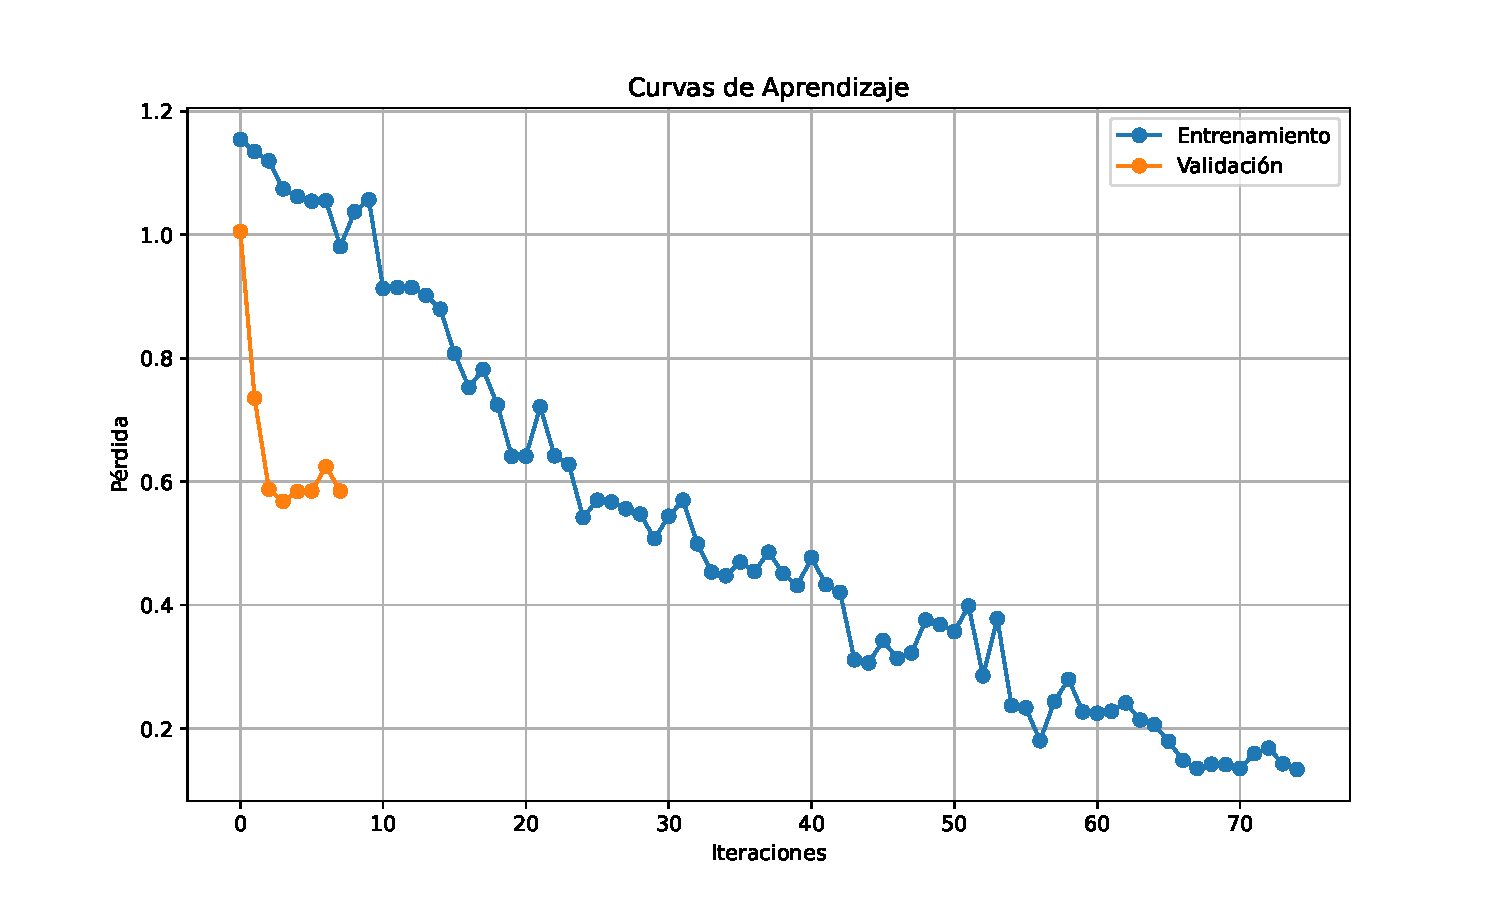
\includegraphics[width=0.65\textwidth]{curvas_de_perdida.pdf}
		\caption{Curva de pérdida durante el entrenamiento y validación.}
		\label{fig:curvaTrain}
	\end{figure}
	
	La gráfica de la función de pérdida de la figura \ref{fig:curvaTrain} muestra una disminución constante tanto en el entrenamiento como en la validación, lo que indica un aprendizaje efectivo y una convergencia adecuada hacia el final de las tres épocas. Además, la ausencia de divergencias entre las curvas sugiere que el modelo no presenta sobreajuste y generaliza bien al conjunto de validación.
	
	
	\section{Conclusiones}
	
	
	
	
	
	\printbibliography
	
	
	
\end{document}